\documentclass[sageh,times]{sagej}
\usepackage{moreverb,url}
%\usepackage[bookmarksopen,bookmarksnumbered,citecolor=black,urlcolor=black]{hyperref}
\newcommand\BibTeX{{\rmfamily B\kern-.05em \textsc{i\kern-.025em b}\kern-.08em
T\kern-.1667em\lower.7ex\hbox{E}\kern-.125emX}}
\def\volumeyear{2017}

\RequirePackage[citecolor=0 0 0,colorlinks=false]{hyperref}
\hypersetup{
     breaklinks=true,
     bookmarksopen=true,
     bookmarksnumbered=true,
     linkcolor=black,
     urlcolor=black,
     citecolor=black,
     colorlinks=true}


%%% The amssymb package provides various useful mathematical symbols
%\usepackage{amssymb}
%%% The amsthm package provides extended theorem environments
% \usepackage{amsthm}
% \usepackage{amsmath}
% \usepackage{color}
% \usepackage{amsmath}
%\usepackage{siunitx}
%\usepackage{framed} % Framing content
%\usepackage{multicol} % Multiple columns environment
%\usepackage{nomencl} % Nomenclature package
%\makenomenclature
%%\setlength{\nomitemsep}{-\parskip} % Baseline skip between items
%\setlength{\nomitemsep}{0.01cm}
%\renewcommand*\nompreamble{\begin{multicols}{2}}
%\renewcommand*\nompostamble{\end{multicols}}
%\newcommand{\degreeC}{\ensuremath{^\circ}C }
\usepackage{eurosym}



\begin{document}

%\begin{frontmatter}
%\title{The Paris end of town? Urban typology through machine learning.} 
%%% use optional labels to link authors explicitly to addresses:
%\author[melb,monash]{Kerry A. Nice}
%\corref{cor1}
%\ead{kerry.nice@unimelb.edu.au}
%\cortext[cor1]{Principal corresponding author}
%
%\author[melb]{Jason Thompson} 
%\author[melb]{Jasper Wijnands} 
%\author[melb]{Gideon Aschwanden} 
%\author[melb]{Mark Stevenson} 
%
%\address[melb]{Transport, Health, and Urban Design Hub, Faculty of Architecture, Building, and Planning, University of Melbourne, Victoria 3010, Australia}
%\address[monash]{School of Earth, Atmosphere and Environment, Monash University, Clayton, Australia}


\runninghead{Nice et al.}
\title{The Paris end of town? Urban typology through machine learning.}

\author{Kerry A. Nice\affilnum{1}, Jason Thompson\affilnum{1}, Jasper Wijnands\affilnum{1}, Gideon Aschwanden\affilnum{1}, and Mark Stevenson\affilnum{1}}

\affiliation{\affilnum{1}Transport, Health, and Urban Design Hub, Faculty of Architecture, Building, and Planning, University of Melbourne, Victoria 3010, Australia}


\corrauth{Kerry A. Nice, Transport, Health, and Urban Design Hub, Faculty of Architecture, Building, and Planning, University of Melbourne, Victoria 3010, Australia}

\email{kerry.nice@unimelb.edu.au}


\begin{abstract}

The confluence of recent advances in availability of geospatial information, computing power, and artificial intelligence offers new opportunities to understand how and where our cities differ and also, how they are alike. Departing from a traditional `top-down' analysis of urban design features, this project analyses thousands of images of urban form (consisting of street view and satellite imagery as well as street maps) from each Australian state and territory capital city, before making comparisons to a group of 20 other high profile cities from around the world including London, Paris, Copenhagen, Beijing, Los Angeles, and New York. We then map these international cities across each Australian example to produce within-city locations that demonstrate the closest connections between these areas and their international comparators. Finally, we suggest relationships between urban design and consequent transport, environmental, and population health outcomes these comparisons suggest may be generated by each location. This work demonstrates an entirely new and highly efficient method for understanding the relationship between cities around the world, and the health, transport, and environmental consequences of their design. Perhaps most importantly, it also answers the age-old question, ``Is there really a `Paris-end' of your city?''.
\end{abstract}

\keywords{machine learning, urban typology, urban design, transport and health}

\maketitle


\section{Introduction}\label{sec:introduction}



 
In 2013, 65\% of Australians lived in capital cities and it is estimated that this will increase to 72\% by 2053  \citep{ABS2008}. These projections are reflected in population growth estimates that will see the country's population likely increase from 24 million today to over 33 million by 2050  \citep{ABS2008}. This growth is expected to mostly take place within the four largest capital cities (Sydney, Melbourne, Brisbane and Perth) with projections indicating that by 2053 both Sydney and Melbourne will have populations of almost 8 million  \citep{CommonwealthofAustralia2010}. As a consequence of this population growth, an array of transportation and population health challenges will emerge.

The importance of integrating transport plans with decisions regarding land-use is being recognised by governments \citep{ATAP2016,SA2015}. Land-use decisions significantly influence transport options and travel choice. Further, the high levels of low-density suburbanisation and high car dependency that characterise many Australian and New Zealand cities are remnants of a mid-twentieth century focus on home and car ownership \citep{Currie2007,Dodson2008}. As a consequence, the status and practical utility of cycling or walking for daily travel requirements is limited \citep{Heesch2014,Daley2011}. Low-density housing renders the cost of large-scale public transport prohibitive, producing a reliance on private vehicles and increasing exposure to risks associated with traffic speed, volume, emissions, and physical inactivity  \citep{Cepeda2016,MingWen2008,Norman2006}. Although some progress has been made in promoting active modes of transport the percentage of Australians walking or cycling to work remains low and primarily concentrated in low-speed, inner-city areas where distances are minimal. Public health policy-makers and urban/transport planners have an opportunity to change this situation by embracing strategies that proactively support active transport modes as facilitated by urban designs witnessed in other countries around the world.

For example, Copenhagen's significant long-term investment in cycling infrastructure of over \euro 30 million in cycling infrastructure for a city of approximately 550,000 residents has seen its rates of cycling mode share expand to 45\% of all trips without consequent increases in road trauma \citep{Kaplan2014}. Similarly, Amsterdam's (and the Netherlands more generally) continued leadership in active transport promotion has demonstrated that cycling and walking can be re-claimed in areas and streets previously lost to car traffic, producing both health and economic benefit \citep{Andersen2000}. Substantial published evidence indicates that land-use affects transport modal choice and behaviour  \citep{Giles-corti2016,Kleinert2016,Goenka2016}. In addition, improved population health outcomes related to chronic conditions such as respiratory disease, cardiovascular disease, and Type 2 diabetes are strongly linked with more active transport modal choices  \citep{Zapata-Diomedi2017}. Therefore, the creation of cities and precincts that facilitate greater uptake of safe, active transport could produce manifold environmental, productivity, and population health benefits. 

However, understanding the association between urban design features and health or environmental outcomes remains difficult, especially when underlying data, locations, methods, and demographics upon which statistical models are built vary considerably across studies. The confluence of recent advances in availability of geospatial information, computing power, and artificial intelligence offers new opportunities to understand how and where our cities differ and also, how they are alike. Departing from a traditional `top-down' analysis of urban design features, this project analyses thousands of images of urban form from each Australian state and territory capital city, before making comparisons to a group of 20 other high profile cities from around the world including London, Paris, Copenhagen, Beijing, Los Angeles, and New York. We then map these international cities across each Australian example to produce within-city locations that demonstrate the closest connections between these areas and their international comparators. Finally, we suggest relationships between urban design and consequent transport, environmental, and population health outcomes these comparisons suggest may be generated by each location.

This work demonstrates an entirely new and highly efficient method for understanding the relationship between cities around the world, and the health, transport, and environmental consequences of their design. Perhaps most importantly, it also answers the age-old question, ``Is there really a `Paris-end' of your city?''.


\section{Methods}\label{sec:methods}

\subsection{Neural network}\label{sec:methods1}














The methods in this study are based on artificial intelligence, in particular deep neural networks \citep{Bishop1995,Samarasinghe2016,Graupe2013}. Neural network architectures that have proven to be particularly successful at image recognition tasks are convolutional neural networks \citep{Schmidhuber2015}. These networks generally consist of alternating layers with convolution operations (for feature identification) and max-pooling operations (improving translation invariance and reducing dimensionality). To increase robustness of these complex models, techniques such as weight regularisation and dropout can be applied \citep{Srivastava2014}.

The model for image recognition used in this study is based on a newer version of the Inception architecture \citep{Szegedy2015}, which demonstrated better computer vision performance than any other methodology during the ImageNet Large-Scale Visual Recognition Challenge (ILSVRC) \citep{Russakovsky2015} in 2014. In particular, we use the third version of Inception (Inception V3) \citep{Szegedy2015a}, achieving even higher performance on ILSVRC by factorising large spatial filters into smaller convolutions, combined with more aggressive regularisation. These Inception models optimise the computational budget required to calibrate the network, while increasing depth and width of the neural network structure to allow for additional complexity.

\subsection{Imagery sampling}\label{sec:methods2}
TODO change this to be about all three

The concept used in this study is to identify a city based on images of its mapped transport network. By classifying images as belonging to a specific city, the model can accurately determine unique features associated with individual city design. 

Cities were selected using a United Nations World Urbanization Prospects list of 1692 cities with greater than 300,000 residents \citep{UN2014}. Google Maps data was used to identify urban form for each of these cities in a globally consistent framework. Due to mapping inconsistencies in South Korea, all 25 South Korean cities were removed from the dataset, reducing the number of cities to 1667. The sampling area for each city was chosen as a circular area aligned to the city's centre, where the radius $r$ (km) of the sampling area was determined based on the population size $p$ according to Bethelemy (2015, Jason TODO):

\begin{equation}
r = \sqrt{ \frac{28.27}{\Pi} \bigg( \frac{p}{300,000}  \bigg)^{0.85} }
\end{equation}

Cities were identified from the 2015 United Nations list of cities with populations exceeding 300,000 residents \citep{UN2014}. 1662 cities were selected, capturing 2.2 billion people or approximately 31\% of the world's population in 2015. Having identified individual cities, a 2-stage sampling approach was applied. Firstly, a sampling area with a centroid derived from the United Nations dataset and with a radius 1.5 km set as a baseline; this was necessary particularly for cities with 300,000 residents (e.g., Christchurch, New Zealand, Izmit, Turkey). As sample cities' populations increased in size, the sampling area then increased by a power of 0.85 to the proportional increase in population size (Bethelemy, 2015). Standardising the sampling area in this manner avoided socio-political discrepancies relating to a city's `true' boundary. Further, it captured differences in population density and shape between cities while also appropriately adjusting for areas of the world's mega-cities namely, cities with populations exceeding 10 million people (e.g., Tokyo, Japan and Delhi, India). Location sampling areas were also adjusted for the earth's curvature at various latitudes using the Haversine approximation of the great circle distance to the city's centre \citep{Sinnott1984}. 

Location sampling is adjusted for the Earth's curvature using the haversine approximation of the great circle distance to the city's centre \citep{Sinnott1984}. Further, large water bodies were removed from this area, since these are not highly indicative of urban form. As a first step, coastlines were identified using the Global Self-consistent Hierarchical High-resolution Geography database, version 2.3.6 \citep{Wessel1996}. Using QGIS \citep{QGIS2009} it was determined whether a sample was located off-shore. Off-shore samples were iteratively replaced by new random samples, preventing downloading images that would not be used. Second, after the initial download, completely blue images were iteratively replaced by a new random sample to remove any lakes. Partly blue images have been retained.

These procedures result in a population and water body-adjusted circular area centred on the city's central coordinates. For example, Figure \ref{fig:hongkong}  shows the resulting sampling locations for Hong Kong.



\begin{figure}[!htbp] 
    \centering    
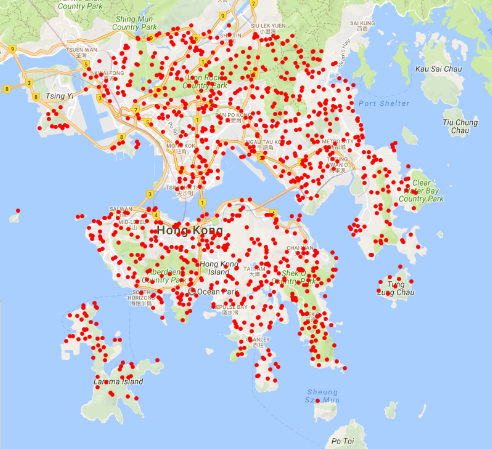
\includegraphics[scale=1]{Images/HongKong.png} 
\caption{Randomly generated locations to sample urban form in Hong Kong.} 
\label{fig:hongkong}  
\end{figure}


\subsection{Imagery sources}\label{sec:methods3}

For each city, three different types of imagery were used to train three neural networks, using street maps, satellite imagery, and street view imagery. It was attempted to use imagery for all 1692 cities, but limitations with each data set meant that less were ultimately used. Python scripts were written to download images according to the methods detailed in Section \ref{sec:methods2} from each of the following sources using the appropriate APIs.

The first neural network used precinct-level Google Maps (GM) images as training material. These were obtained from the selected locations using a custom style defined with the Google Static Maps API \citep{GoogleStatic2017} (see Figure \ref{fig:maps} for examples of Paris, France). The images, sized 320 by 320 pixels, provide a high-level abstraction of road (black) and public transport (orange) networks, green space (green), and water bodies (blue). Any remaining space is coded white. Images were taken from 1665 cities using 1,665,000 images. 

\begin{figure}[!htbp]
    \centering    
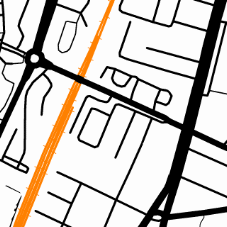
\includegraphics[scale=1]{Images/Map1.png} 
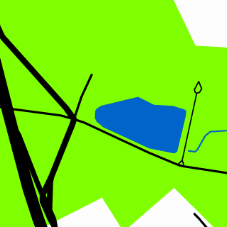
\includegraphics[scale=1]{Images/Map2.png} 
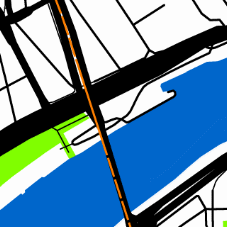
\includegraphics[scale=1]{Images/Map3.png} 
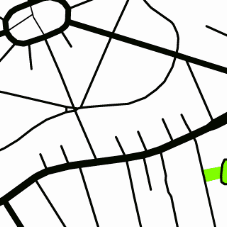
\includegraphics[scale=1]{Images/Map4.png}  
\caption{Four sample GM images for Paris, France \citep{GoogleStatic2017}}    
 \label{fig:maps}  
\end{figure} 

The second type of imagery, Google Satellite (GS) imagery used was obtained using the Google Static Maps API \citep{GoogleStatic2017}. Image type was set to `satellite', zoom level of 16, image size of 256x256. Training samples of 1000 images per city were taken for 1688 cities for a total of 1,688,000 images. Figure \ref{fig:satbeiade} shows four sample images, two each of Adelaide, Australia and Beijing, China. 


\begin{figure}[!htbp]
    \centering    
\includegraphics[scale=0.30]{Images/Satellite/{Adelaide,Australia_0_-34.892090,138.603093}.png} 
\includegraphics[scale=0.30]{Images/Satellite/{Adelaide,Australia_0_-34.893723,138.582879}.png} 
\includegraphics[scale=0.30]{Images/Satellite/{Beijing,China_0_39.763402,116.457312}.png} 
\includegraphics[scale=0.30]{Images/Satellite/{Beijing,China_0_39.783779,116.531780}.png} 
\caption{Sample GS images for Adelaide, Australia and Beijing, China. \citep{GoogleStatic2017}}    
 \label{fig:satbeiade}  
\end{figure} 

The third imagery type was street view imagery obtained through a combination of Google Street View (GSV) \citep{GoogleMaps2017b} and Baidu Maps Street View (BSV) \citep{Baidu2017}. 1000 images were sampled for 1074 cities (for a total of 1,074,000 images) at a 256x256 resolution with a pitch of 0, a field of view of 90 degrees and a random heading. Images inside tunnels, indoor locations, or dark locations were manually removed and more images sampled to bring each city's total up to 1000 again.

No street view imagery of China is available through GSV, so BSV was used to supplement.  In order to minimise the differences between the two data sources as well as to minimise strong country-specific items (i.e. text on road signs) influencing the neural network training, further image processing was performed to segment each image before using the images in training and evaluation. The Python module \textit{pymeanshift} \citep{Pymeanshift2017} was used to segment each image, using a spatial radius of 6, range radius of 4.5, and minimum density of 50. Figure \ref{fig:gsvbsv} shows an example of an original GSV image (of Sydney, Australia) and its segmented version as well as an original BSV image (of Beijing, China) and its segmented version.

\begin{figure}[!htbp]
 %   \centering    
 \includegraphics[scale=0.30]{Images/SydStreetView/{9990_-33.806205549999845_150.939042099999940}.jpg} 
 \includegraphics[scale=0.30]{Images/SydSegStreetView/{9990_-33.806205549999845_150.939042099999940}.jpg} 
    \includegraphics[scale=0.30]{Images/ChinaBSV/{Beijing,China_0_39.785332,116.345079}.jpg} 
   \includegraphics[scale=0.30]{Images/ChinaBSVSeg/{Beijing,China_0_39.78533,116.345079}.jpg} 
 \\ \tiny  a) ~~~~~~~~~~~~~~~~~~~~~~~~~~~~~~~~~~~~~~~~~~~~~~~~~~~~~~~~~~ b) ~~~~~~~~~~~~~~~~~~~~~~~~~~~~~~~~~~~~~~~~~~~~~~~~~~~~~~~~~~  c) ~~~~~~~~~~~~~~~~~~~~~~~~~~~~~~~~~~~~~~~~~~~~~~~~~~~~~~~~~~ d)
\caption{Sample GSV image from Sydney, Australia (a) \citep{GoogleMaps2017b} and the processed segmented version (b). Sample BSV image from Beijing, China (c) \citep{Baidu2017} and the processed segmented version (d).}    
 \label{fig:gsvbsv}  
\end{figure} 

%Melbourne maps 22996
%Sydney maps 24589
%Melbourne satellite 23027
%Sydney satellite 24596
%Melbourne street 20971
%Sydney street 14644

Images from Sydney and Melbourne, Australia were excluded from the training data sources for the three neural networks described above and were instead sampled as evaluation data. This evaluation data was sampled at a 400m grid resolution across the greater metro areas, with 23027 points for Melbourne and 24596 points for Sydney (of which images available through GSV were 20971 and 14644 for Melbourne and Sydney respectively). Each of these evaluation data sets were downloaded through the same process and the training data sets above (and using the same image segmentation post-processing for GSV images).



 \subsection{Neural network training}\label{sec:methods4}    

To accurately calibrate the 25 million parameters of the Inception V3 architecture for any computer vision task, it is preferable to use millions of training images with high-quality labels. Therefore, 1000 samples were randomly selected from each city area, resulting in a study dataset of 1,667,000 images. This dataset, obtained using Python \citep{Python2016}, was randomly split into a training (75\%) and validation (25\%) set. In order to obtain a balanced training data set of 750 images per city, sampling was performed sequentially per city.
The Inception V3 network was calibrated using supervised learning with the generated dataset to identify the name of the city based on a supplied precinct-level image. Several pre-processing steps were performed before supplying the image to the neural network. In particular, images were randomly flipped and randomly cropped during pre-processing from 320x320x3 to Inception V3's native 299x299x3 resolution. No zooming is applied and the aspect ratio is kept fixed, while colour transformations are not required due to our pre-specified limited colour scheme. All images were normalised to [-1, 1] by subtracting a colour value of 128 from each pixel and multiplying by 1/128. To ensure good mixing, training images were randomly allocated to batches. Validation images were transformed to 299x299x3 using central cropping.

To update weights in the neural network, a loss function has to be specified to quantify the extent of any current misclassifications. The loss function used in this study is a weighted sum of the cross entropy calculated on the softmax function output of the nodes in the final layer (77\%) and the auxiliary end nodes (23\%). Model parameters are calibrated by minimising this loss function using Stochastic Gradient Descent with Nesterov momentum of 0.9. Other parameters include a batch size of 64 samples, learning rate starting at 0.9 per batch, reduced by 6\% every two epochs, batch normalization, a dropout rate of 0.2 after the final average-pooling operations, and an L2 regularization weight per sample of 0.0001. After Glorot uniform random weight initialisation, the model was trained until convergence for a total of 150 epochs (approximately one to two weeks using one NVIDIA GTX 1080 GPU), using the Microsoft Cognitive Toolkit (CNTK) \citep{Yu2015}. 

This process resulted in three trained models. The model for GM reached a validation accuracy of 85.375\% and top 5 error of 7.705\%. The model for GS reached a validation accuracy of 99.419\% and top 5 error of 0.032\%. The model for GSV-BSV reached a validation accuracy of 43.123\% and top 5 error of 30.186\%.

%GM
%GS
%GSV-BSV
%
%
%This resulted in 86.1\% accuracy of the final model for predicting the correct city using images in the validation set (i.e., top 1 error of 13.9\%). Inference of each of the 416,750 images in the validation set also resulted in probability estimates for all 1667 classes the image could belong to. These probability estimates were used in graph-based clustering as follows.
%
%
%% maps Finished Epoch[150 of 150]: [Validate] ce = 0.75979399 * 416250; errs = 14.625% * 416250; top5Errs = 7.705% * 416250
%% Satellite Finished Epoch[150 of 150]: [Validate] ce = 0.02372664 * 422500; errs = 0.581% * 422500; top5Errs = 0.032% * 422500
%% Street view results_per_epoch_Minus_SydMel.2:Finished Epoch[150 of 150]: [Validate] ce = 2.69203455 * 268280; errs = 56.877% * 268280; top5Errs = 30.186% * 268280
%
%\subsubsection{Maps}
%Imagery from Google Maps was used to train CNTK. Training was run for 150 epochs with the validation step reaching an error rate of 14.625\% (accuracy rate of 85.375\%).
%Imagery from Google Satellite was used to train CNTK. Training was run for 150 epochs with the validation step reaching an error rate of 0.581\% (accuracy rate of 99.419\%). 
%Imagery from Google Street View was used to train CNTK. Training was run for 150 epochs with the validation step reaching an error rate of 56.877\% (accuracy rate of 43.123\%). 



\subsection{Neural network inference}\label{sec:methods5}    
Finally, using the three trained models, inference was performed using the three evaluation data sets for Melbourne and Sydney. As Melbourne and Sydney are not present in the training data, the neural network predictions would choose the city with the most similar characteristics for each of the sampled locations. Using these predictions, every location in both cities can be determined to be `most like' some other world city due to map characteristics, or satellite or street view imagery.





\section{Results}\label{sec:results}



The resulting predictions from performing the inference of the three evaluation data sets by the three trained neural networks were analysed in a number of different ways. The top 20 predicted cities for the evaluation points for each imagery data set were calculated. These top 20 predictions for GM are presented in Table \ref{tab:melbournesydneyGM}, GS in Table \ref{tab:melbournesydneyGS}, and GSV-BSV in Table \ref{tab:melbournesydneyGSV}.

The predictions through GM (Table \ref{tab:melbournesydneyGM}) are dominated by other Australian cities (Brisbane, Canberra, Sunshine Coast, Perth, Newcastle and Lake Macquarie, and Adelaide) as well as a number of cities from Israel, South Africa, and the United States. Australian cities make up nearly 33\% of the top 20 predictions for Melbourne and 32\% for Sydney. Melbourne and Sydney also show strong similarities with each other, sharing 12 common predictions in the top 20 between them.

\begin{table}[!htbp]
\caption{Top 20 cities like Melbourne and Sydney through GM \label{tab:melbournesydneyGM}}     
\begin{tabular}{| l | l |l| l | l|}
\hline
 \hline    &  \multicolumn{2}{c|}{\textbf{Melbourne evaluation}} & \multicolumn{2}{c|}{\textbf{Sydney evaluation}}  \\  
\textbf{Predicted city} & \textbf{Matches} & \textbf{\% matching}  & \textbf{Matches} & \textbf{\% matching}\\ \hline
Brisbane, Australia & 4061 & 17.64 & 3591 & 14.60      \\ \hline
Canberra, Australia & 1699 & 7.38  & 1972 & 8.02     \\ \hline
Beer Sheva, Israel & 1110 & 4.82  & 1989 & 8.09   \\ \hline
Sunshine Coast, Australia & 793 & 3.44  & 364 & 1.48 \\ \hline
Valpara\'{i}so, Chile & 751 & 3.26  & 434 & 1.76 \\ \hline
Haifa, Israel & 563 & 2.44  & 1066 & 4.33 \\ \hline
McAllen, United States of America & 442 & 1.92  &-&- \\ \hline
Auckland, New Zealand & 330 & 1.43  & 208 & 0.85 \\ \hline
Adelaide, Australia & 308 & 1.34  & 326 & 1.33 \\ \hline
Perth, Australia & 287 & 1.25  & 132 & 0.54 \\ \hline
Johannesburg, South Africa & 244 & 1.06  &-&- \\ \hline
Newcastle and Lake Macquarie, Australia & 245 & 1.06  & 1318 & 5.36   \\ \hline
Washington, D.C., United States of America & 198 & 0.86  &-&- \\ \hline
Toronto, Canada & 140 & 0.61  & 151 & 0.61 \\ \hline
Port Elizabeth, South Africa & 138 & 0.6  &-&- \\ \hline
Effon Alaiye, Nigeria & 133 & 0.58  &-&- \\ \hline
Gold Coast, Australia & 132 & 0.57  & 163 & 0.66 \\ \hline
Pretoria, South Africa & 131 & 0.57  &-&- \\ \hline
Louisville, United States of America & 127 & 0.55  &-&- \\ \hline
Tel Aviv-Jaffa, Israel & 126 & 0.55  &-&- \\ \hline
Kiev, Ukraine &-&- & 351 & 1.43\\ \hline
Tasikmalaya, Indonesia&-&- & 344 & 1.40\\ \hline
Caruaru, Brazil &-&- & 241 & 0.98\\ \hline
London, United Kingdom &-&- & 175 & 0.71\\ \hline
Jerusalem, Israel&-&- & 143 & 0.58\\ \hline
London, Canada &-&-& 132 & 0.54\\ \hline
Shantou, China&-&- & 130 & 0.53\\ \hline
West Yorkshire, United Kingdom&-&- & 131 & 0.53\\ \hline
\end{tabular}
\end{table}

The results for the predictions through GS (Table \ref{tab:melbournesydneyGS}) show wider divergences from both Australia and between Melbourne and Sydney. Both Melbourne and Sydney are strongly matched to Brazil. Melbourne is matched to Brazil in 39.5\% of the evaluation locations (and 43.6\% for Brazil and Argentina) while Sydney is matched to Brazil in 50.3 of the evaluation locations (and 54.4\% for Brazil and Argentina). Melbourne and Sydney show wider divergences from each other, only having 7 of the top 20 predicted cities in common. Melbourne shows a stronger connection to Wellington, NZ while Sydney is much more similar to Sevastopol, Ukraine.

\begin{table}[!htbp]
\caption{Top 20 cities like Melbourne and Sydney through GS \label{tab:melbournesydneyGS}}     
\begin{tabular}{| l | l |l| l | l|}
\hline
 \hline    &  \multicolumn{2}{c|}{\textbf{Melbourne evaluation}} & \multicolumn{2}{c|}{\textbf{Sydney evaluation}}  \\  
\textbf{Predicted city} & \textbf{Matches} & \textbf{\% matching}  & \textbf{Matches} & \textbf{\% matching}\\ \hline
Jundia\'{i}, Brazil & 6509 & 28.27 & 6478 & 26.34 \\ \hline
Wellington, NZ & 3124 & 13.57 & 161 & 0.65 \\ \hline
Adelaide, Australia & 1624 & 7.05 &-&- \\ \hline
Campinas, Brazil & 1408 & 6.11 & 4088 & 16.62 \\ \hline
Miami, United States of America & 1095 & 4.76 &-&- \\ \hline
Provo-Orem, United States of America & 1022 & 4.44 &-&- \\ \hline
Macap\'{a}, Brazil & 614 & 2.67 &-&- \\ \hline
Rosario, Argentina & 542 & 2.35 & 1006 & 4.09 \\ \hline
Gold Coast, Australia & 463 & 2.01 &-&- \\ \hline
Catania, Italy & 410 & 1.78 &-&- \\ \hline
Juiz De Fora, Brazil & 411 & 1.78 & 1481 & 6.02 \\ \hline
Buenos Aires, Argentina & 392 & 1.7 &-&- \\ \hline
Canberra, Australia & 372 & 1.62 & 170 & 0.69 \\ \hline
Palma, Spain & 323 & 1.4 &-&- \\ \hline
Newcastle and Lake Macquarie, Australia & 274 & 1.19 & 152 & 0.62 \\ \hline
Sunshine Coast, Australia & 228 & 0.99 &-&- \\ \hline
Surakarta, Indonesia & 214 & 0.93 &-&- \\ \hline
Johannesburg, South Africa & 212 & 0.92 &-&- \\ \hline
Palm Bay-Melbourne, United States of America & 176 & 0.76 &-&- \\ \hline
Bel\'{e}m, Brazil & 169 & 0.73 &-&- \\ \hline
Sevastopol, Ukraine &-&- & 3360 & 13.66\\ \hline
Belgaum, India &-&- & 1177 & 4.79\\ \hline
Memphis, United States of America &-&- & 604 & 2.46\\ \hline
Baaqoobah, Iraq &-&- & 442 & 1.8\\ \hline
Nagasaki, Japan &-&- & 359 & 1.46\\ \hline
Qazvin, Iran &-&- & 303 & 1.23\\ \hline
Guayaquil, Ecuador &-&- & 216 & 0.88\\ \hline
Malaga, Spain &-&- & 201 & 0.82\\ \hline
Campos dos Goytacazes, Brazil &-&- & 197 & 0.8\\ \hline
Guangyuan, China &-&- & 147 & 0.6\\ \hline
New Orleans, United States of America &-&- & 147 & 0.6\\ \hline
Chiinu, Republic of Moldova &-&- & 146 & 0.59\\ \hline
Baixada Santista, Brazil &-&- & 135 & 0.55\\ \hline
\end{tabular}
\end{table}

Finally, the predictions through GSV-BSV (Table \ref{tab:melbournesydneyGSV}) show stronger similarities between Melbourne and Sydney than the previous two data sources. In the Melbourne evaluation, just over 30\% (7 of the top 8 picks) are other Australian cities, while Sydney matched other Australian cities for 34.6\% of the evaluation locations (and were 7 of the top 7 picks). In addition, 16 of the top 20 predicted cities are shared between Melbourne and Sydney. 

\begin{table}[!htbp]
\caption{Top 20 cities like Melbourne and Sydney through GSV-BSV \label{tab:melbournesydneyGSV}}     
\begin{tabular}{| l | l |l| l | l|}
\hline
 \hline    &  \multicolumn{2}{c|}{\textbf{Melbourne evaluation}} & \multicolumn{2}{c|}{\textbf{Sydney evaluation}}  \\  
\textbf{Predicted city} & \textbf{Matches} & \textbf{\% matching}  & \textbf{Matches} & \textbf{\% matching}\\ \hline
Perth, Australia & 1424 & 6.79 & 497 & 3.39 \\ \hline
Adelaide, Australia & 1349 & 6.43 & 346 & 2.36 \\ \hline
Sunshine Coast, Australia & 1344 & 6.41 & 1139 & 7.78 \\ \hline
Auckland, New Zealand & 930 & 4.43 & 242 & 1.65 \\ \hline
Canberra, Australia & 714 & 3.4 & 770 & 5.26 \\ \hline
Newcastle and Lake Macquarie, Australia & 669 & 3.19 & 789 & 5.39 \\ \hline
Gold Coast, Australia & 470 & 2.24 & 702 & 4.79 \\ \hline
Brisbane, Australia & 384 & 1.83 & 828 & 5.65 \\ \hline
Curitiba, Brazil & 379 & 1.81 & 131 & 0.89 \\ \hline
Stockton, United States of America & 366 & 1.75 & 184 & 1.26 \\ \hline
Christchurch, New Zealand & 339 & 1.62 &-&- \\ \hline
Concord, United States of America & 330 & 1.57 & 131 & 0.89 \\ \hline
Cape Town, South Africa & 285 & 1.36 & 132 & 0.9 \\ \hline
Bonita Springs-Naples, United States of America & 274 & 1.31 & 141 & 0.96 \\ \hline
Teeside , United Kingdom & 262 & 1.25 &-&- \\ \hline
East London, South Africa & 253 & 1.21 & 150 & 1.02 \\ \hline
West Yorkshire, United Kingdom & 248 & 1.18 &-&- \\ \hline
Los Angeles, United States of America & 203 & 0.97 &-&- \\ \hline
San Diego, United States of America & 197 & 0.94 & 300 & 2.05 \\ \hline
Vereeniging, South Africa & 188 & 0.9 & 145 & 0.99 \\ \hline
Jacksonville, Florida, United States of America  &-&- & 156 & 1.07\\ \hline
Virginia Beach, United States of America  &-&- & 152 & 1.04\\ \hline
McAllen, United States of America&-&- & 123 & 0.84\\ \hline
Corpus Christi, United States of America&-&- & 97 & 0.66\\ \hline

\end{tabular}
\end{table}




The predicted output for the three neural networks were plotted on maps of Melbourne and Sydney. To allow a visual identification of geographically similar predictions, the color scheme for the plotted points was determined by the latitude and longitude of the predicted city. This color scheme is shown in Figure \ref{fig:colorscheme}. Using this latitude/longitude color scheme, plots were made for both Melbourne and Sydney for all three neural networks.

\begin{figure}[!htbp]
\centering    
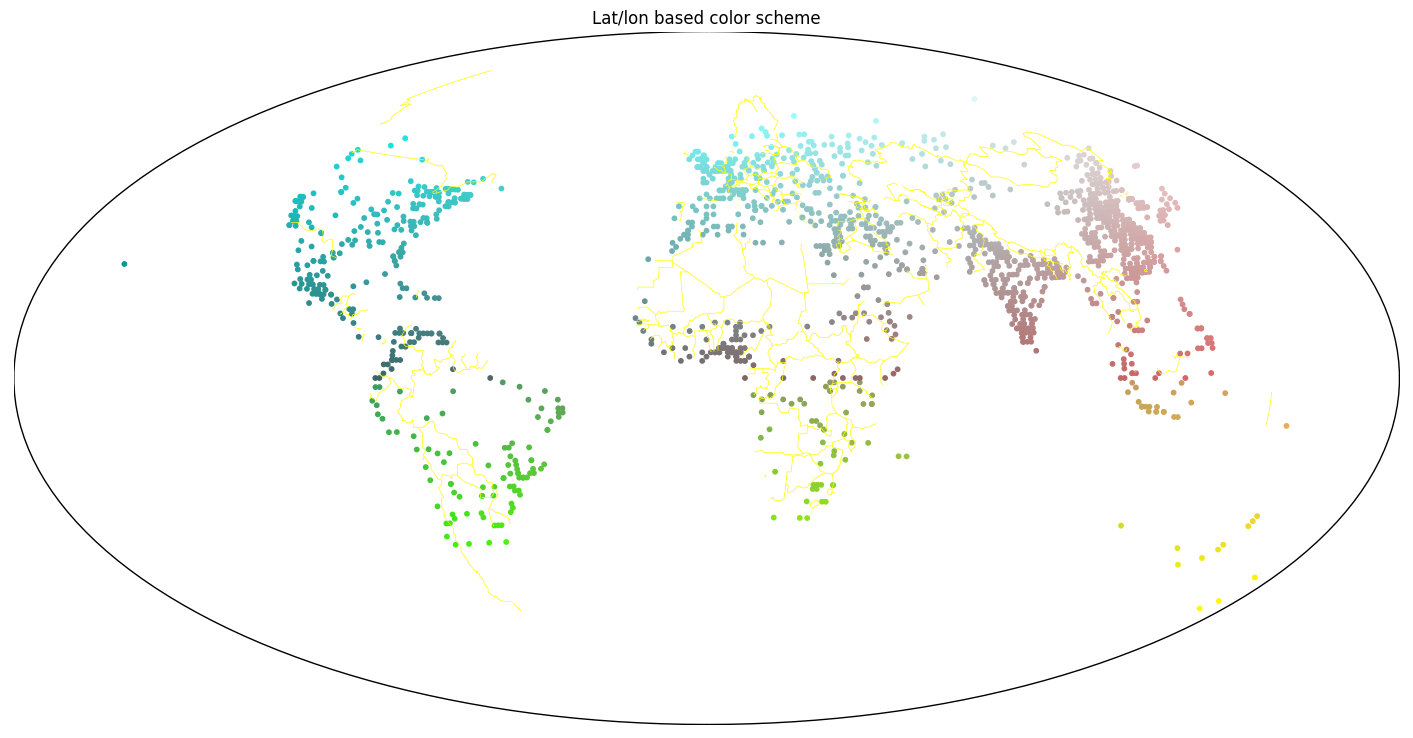
\includegraphics[scale=0.25]{Images/World_map_color_scheme.png} 
\caption{Latitude/longitude based color scheme for plotting matching cities.}    
 \label{fig:colorscheme}  
\end{figure} 


Figure \ref{fig:melmaps} shows all cities plotted against the Melbourne evaluation locations as well as the top 42 predicted locations for the GM neural network. The other Australian cities show a strong grouping in the inner and outer suburbs while the CBD region shows no single strong grouping of regions or specific cities. In Melbourne's far outer suburbs and rural areas shows a wide mix of North and South American, South African, European, and Mid-Eastern cities with small localized clusters of each. In the central business district (CBD), a few locations are predicted as Paris, France (see detail of CBD in Figure \ref{fig:melmapscbd} and \ref{fig:gm_melsyd_paris}), mostly associated with the Docklands or parklands.

  
\begin{figure}[!htbp]
\centering    
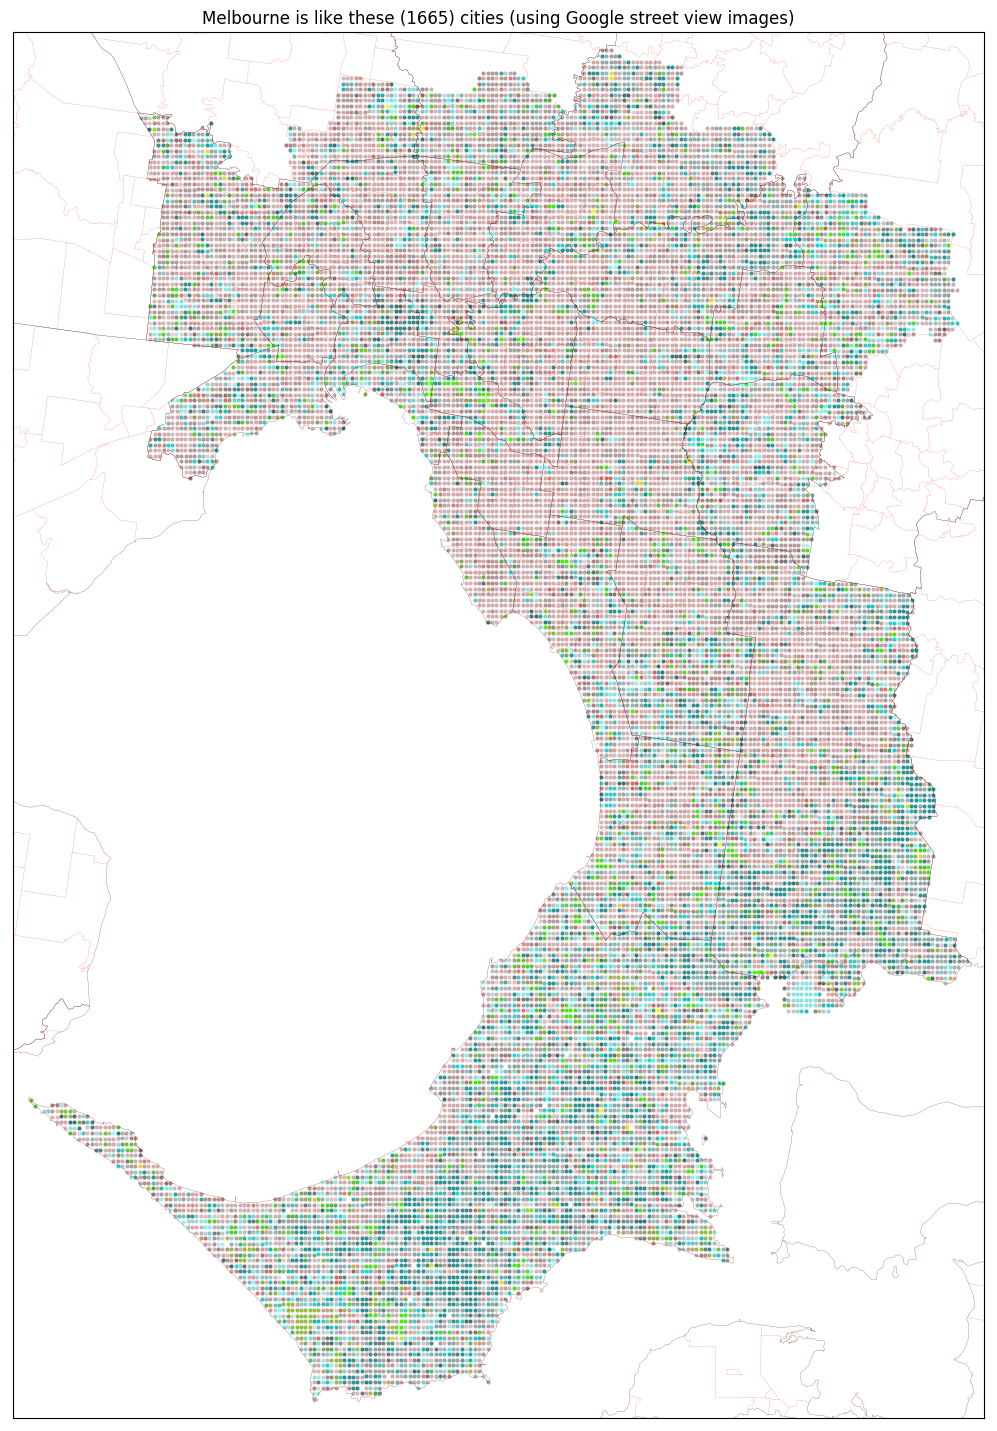
\includegraphics[scale=0.20]{Images/MelbourneOverall_maps.png} 
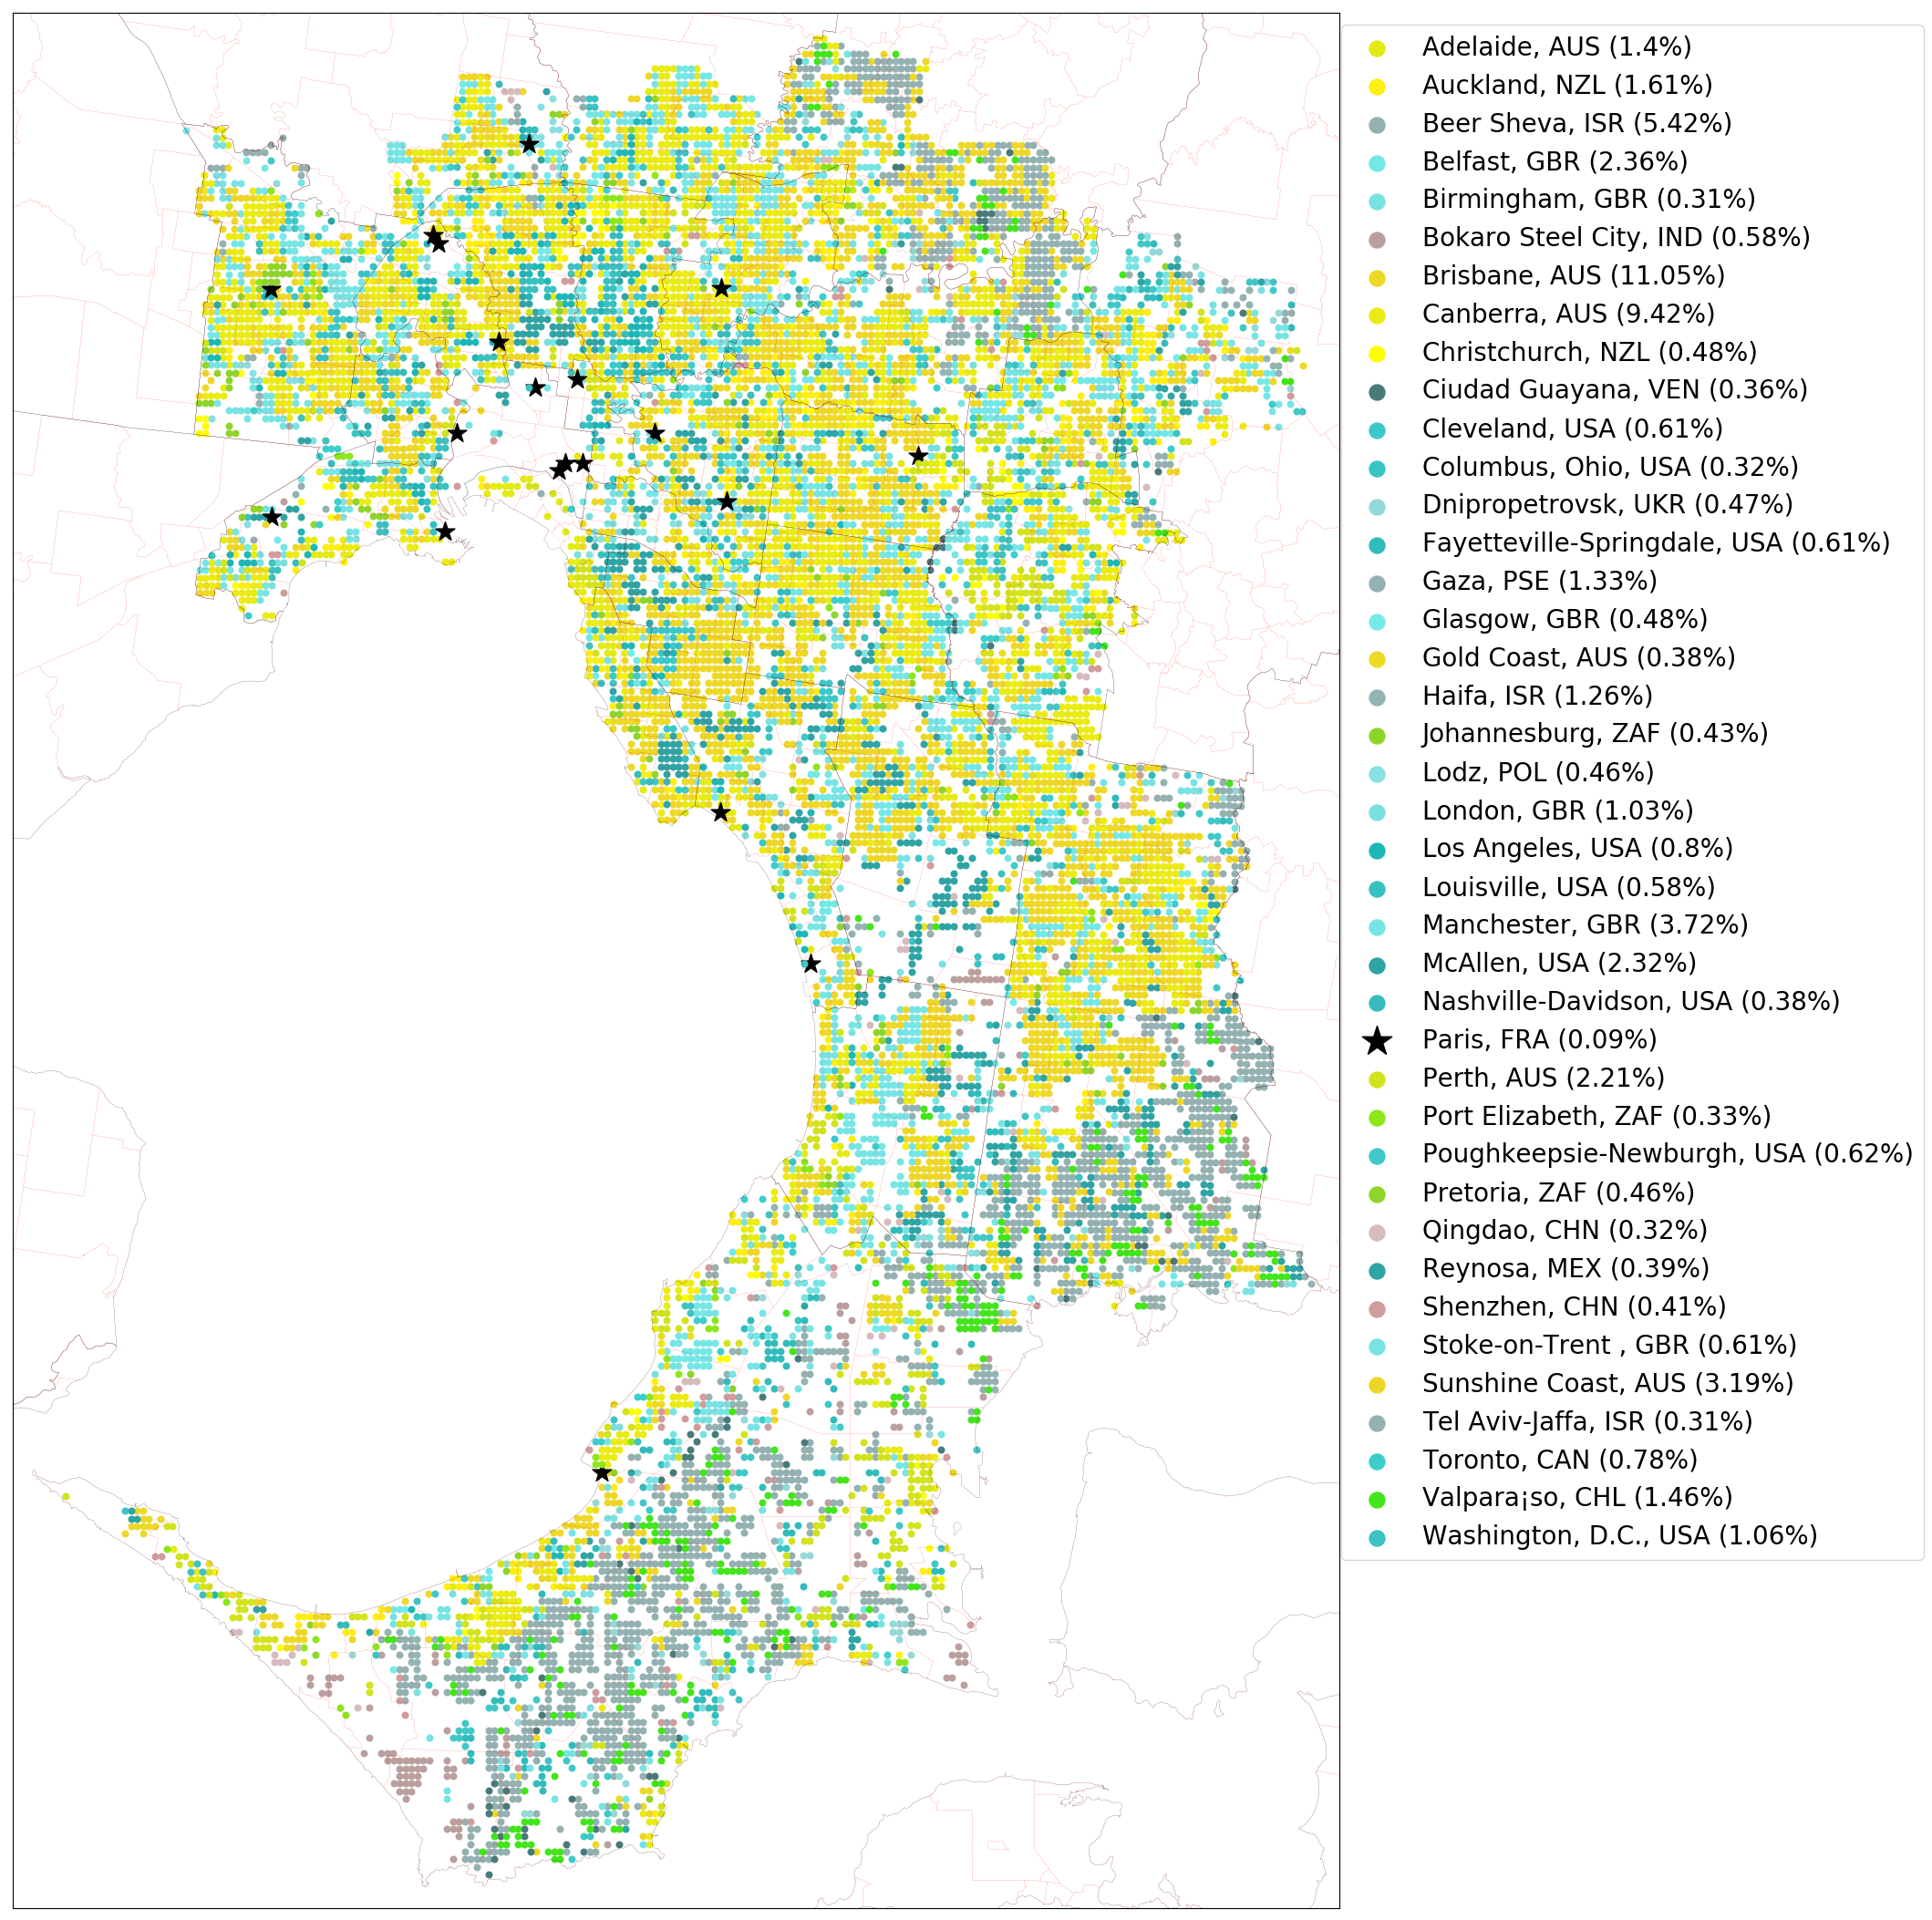
\includegraphics[scale=0.20]{Images/MelbourneOverallAbrev_maps.png} 
\caption{Predicted similar cities using GM neural network for Melbourne evaluation locations. All 1665 cities plotted using Figure \ref{fig:colorscheme} color scheme (left) and top 42 predicted cities (right)}    
 \label{fig:melmaps}  
\end{figure} 

\begin{figure}[!htbp]
\centering     
\includegraphics[scale=0.40]{Images/MelbourneCBD_maps_detail3.png} 
\caption{Predicted similar cities (showing three letter country code of city location) using GM neural network for Melbourne evaluation locations. Detail of Melbourne CBD, with predictions of Paris highlighted in red.}    
 \label{fig:melmapscbd}  
\end{figure} 

Figure \ref{fig:sydmaps} shows all cities plotted against the Sydney evaluation locations as well as the top 42 predicted locations for the GM neural network. Australian cities show up stronger in the western and south eastern suburbs and North American and European cities in the northern and southern suburbs. The CBD and the central parts of the city show less single city or regional groupings but with stronger highly localized clusters of each. Some cities commonly represented in the CBD include Hong Kong, London, Toulon, and Kaohsiung (many cities with waterfronts). Paris, France is predicted in a number of scattered locations across Sydney (see Figure \ref{fig:gm_melsyd_paris}).

\begin{figure}[!htbp]
\centering    
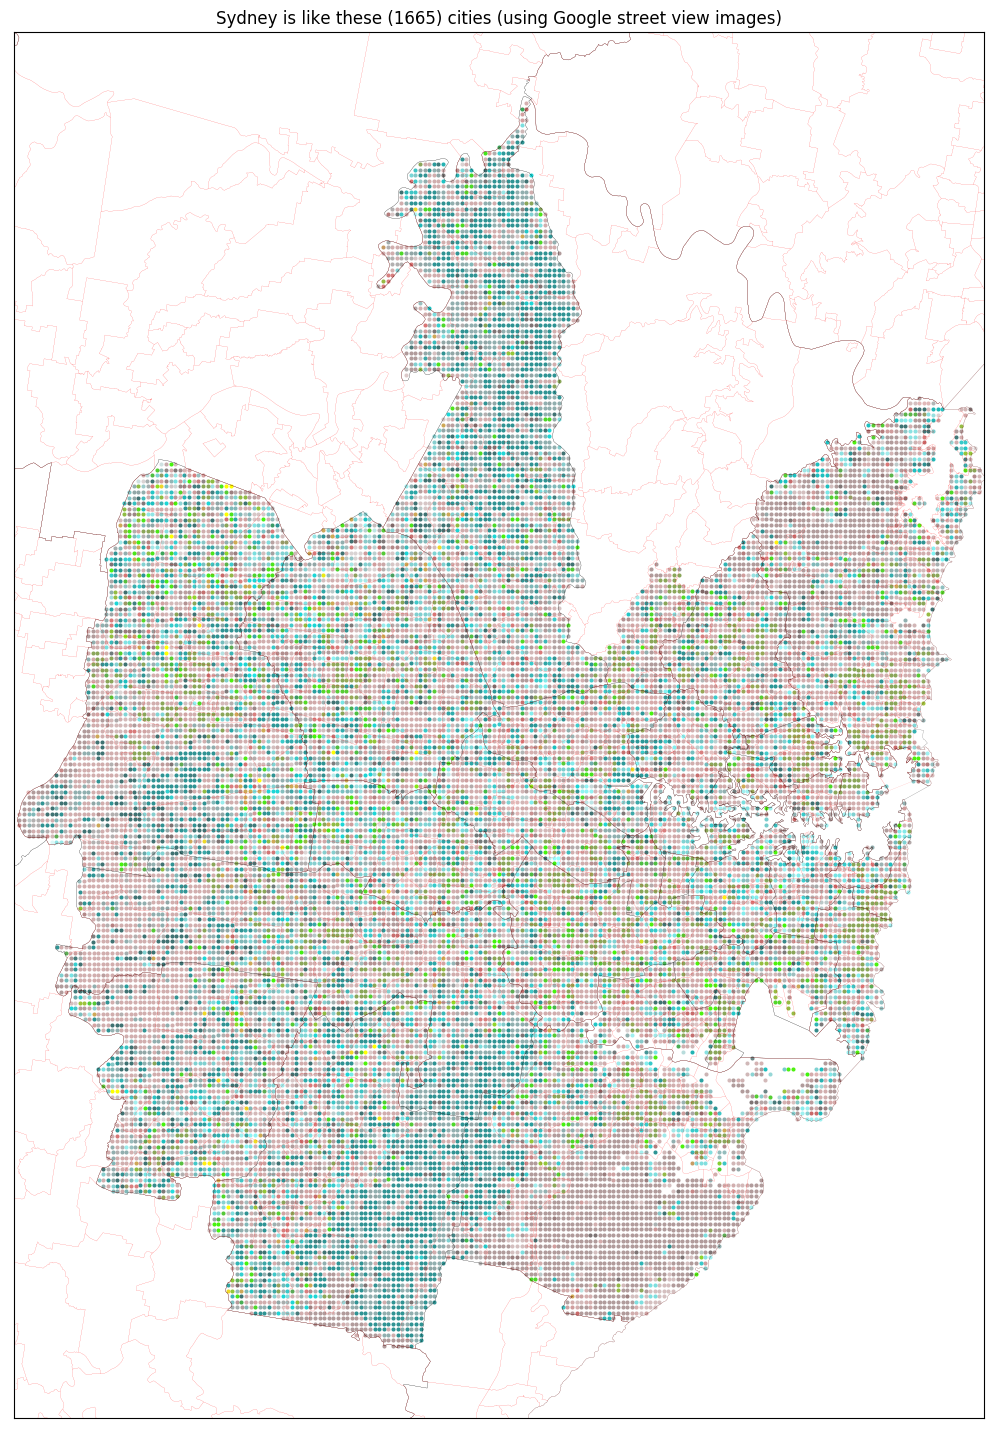
\includegraphics[scale=0.20]{Images/SydneyOverall_maps.png} 
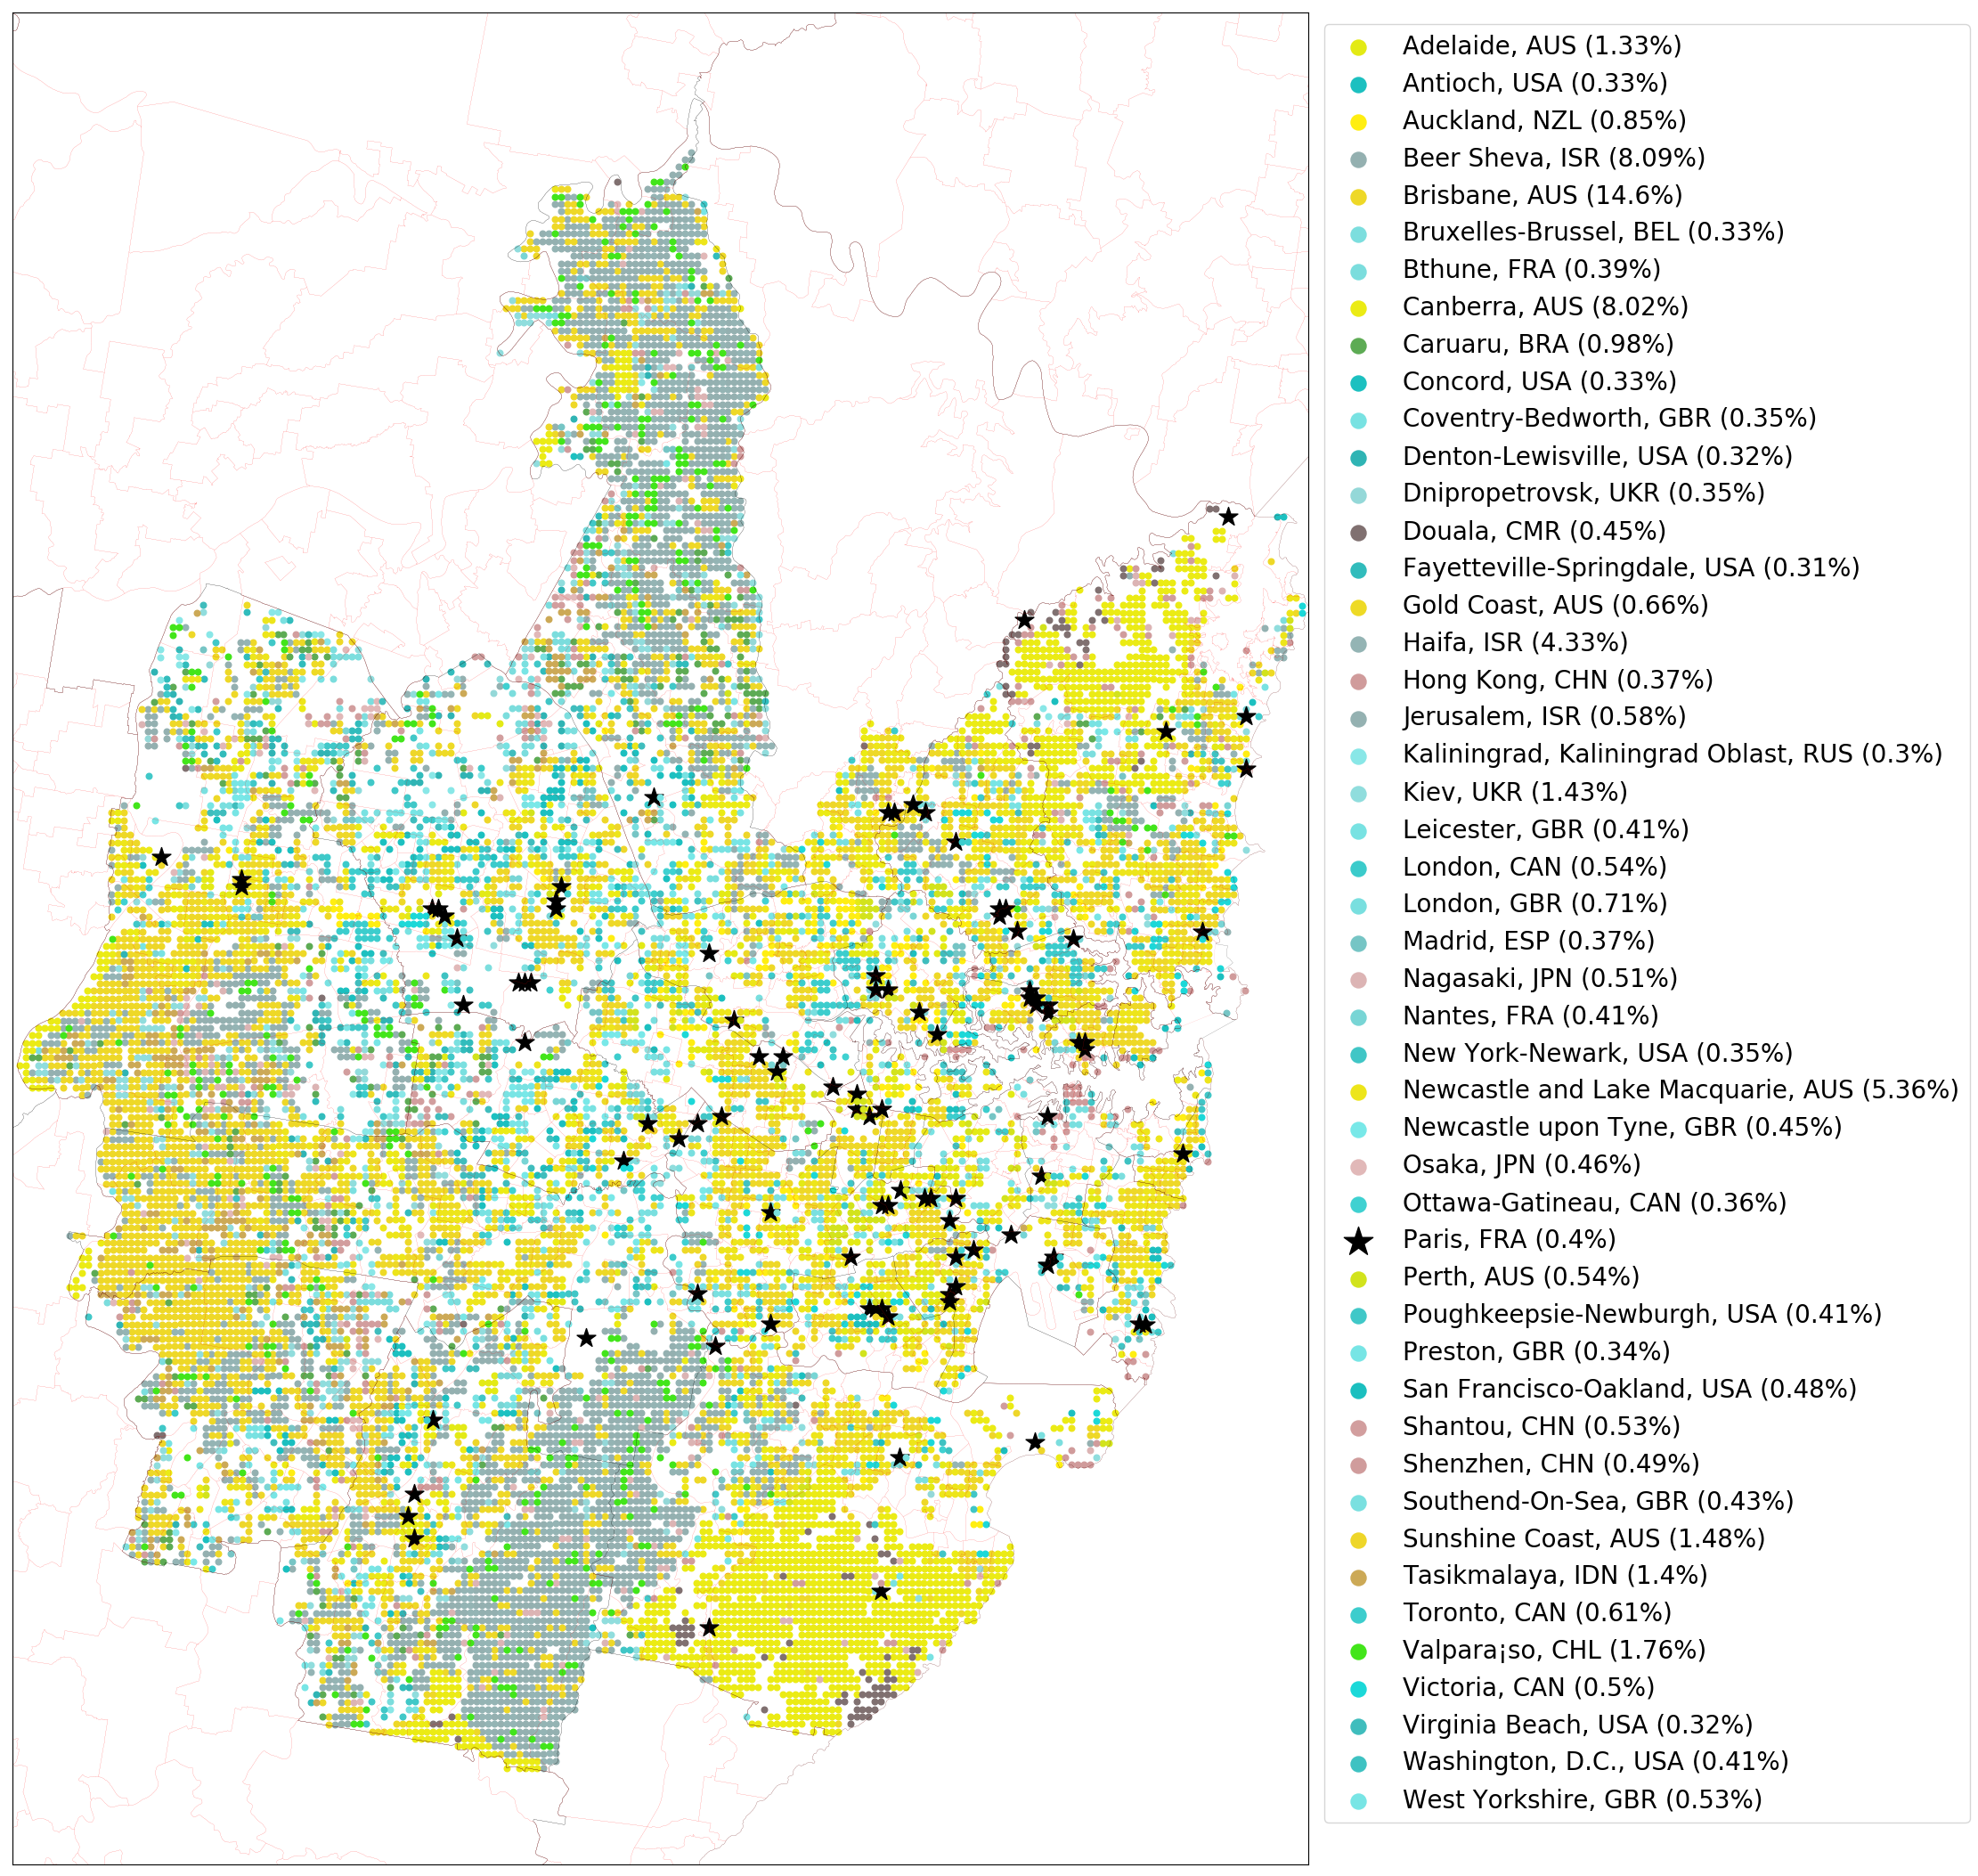
\includegraphics[scale=0.20]{Images/SydneyOverallAbrev_maps.png}  
\caption{Predicted similar cities using GM neural network for Sydney evaluation locations. All 1665 cities plotted using Figure \ref{fig:colorscheme} color scheme (left) and top 42 predicted cities (right)}    
 \label{fig:sydmaps}  
\end{figure} 

\begin{figure}[!htbp]
\centering    
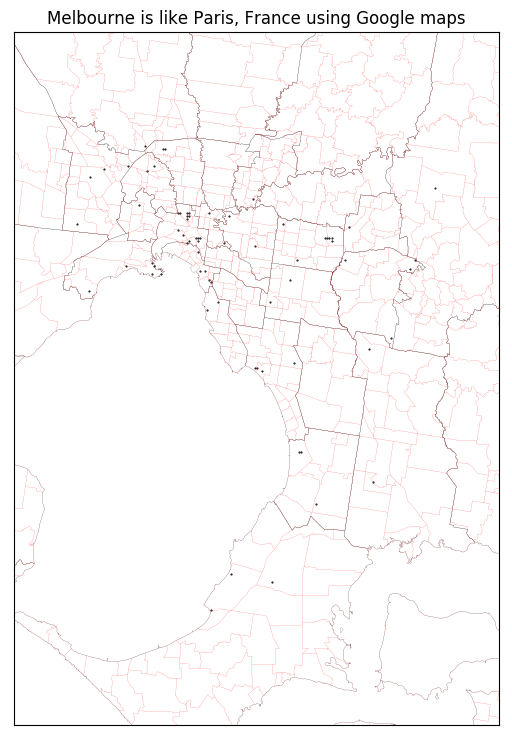
\includegraphics[scale=0.40]{Images/Melbourne_Paris,France-GM.png} 
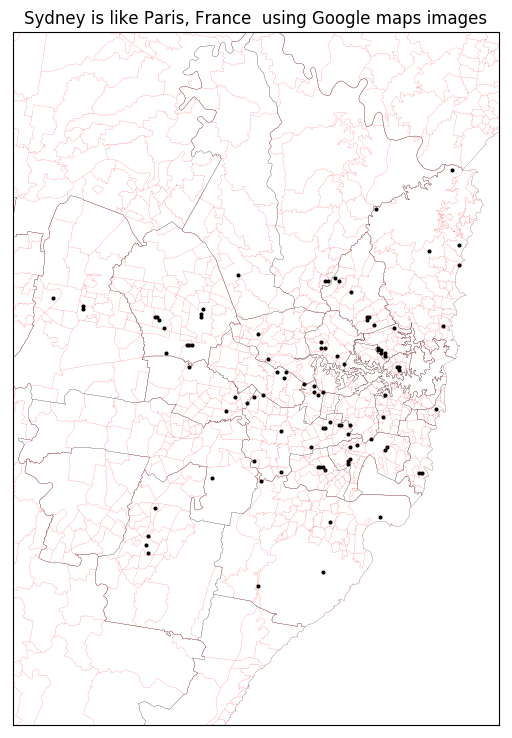
\includegraphics[scale=0.40]{Images/Sydney_Paris,France-GM.png} 
\caption{Distribution of Paris predictions in Melbourne and Sydney using GM.}    
 \label{fig:gm_melsyd_paris}  
\end{figure} 

Figure \ref{fig:melsat} shows all cities plotted against the Melbourne evaluation locations as well as the top 48 predicted locations for the GS neural network. The other Australian cities show a strong grouping in the inner and outer suburbs while the CBD region shows no single strong grouping of regions or specific cities but with a range of predictions such as Miami, United States and Mendoza, Argentina. In Melbourne's far outer suburbs and rural areas shows a wide mix of North and South American (USA, Brazil, and Argentina), South African, European (Italy and Spain), and Mid-Eastern (Iran and Turkey) cities with small localized clusters of each. No predictions of Paris, France have been made by the GS neural network for any evaluation location.





\begin{figure}[!htbp]
\centering    
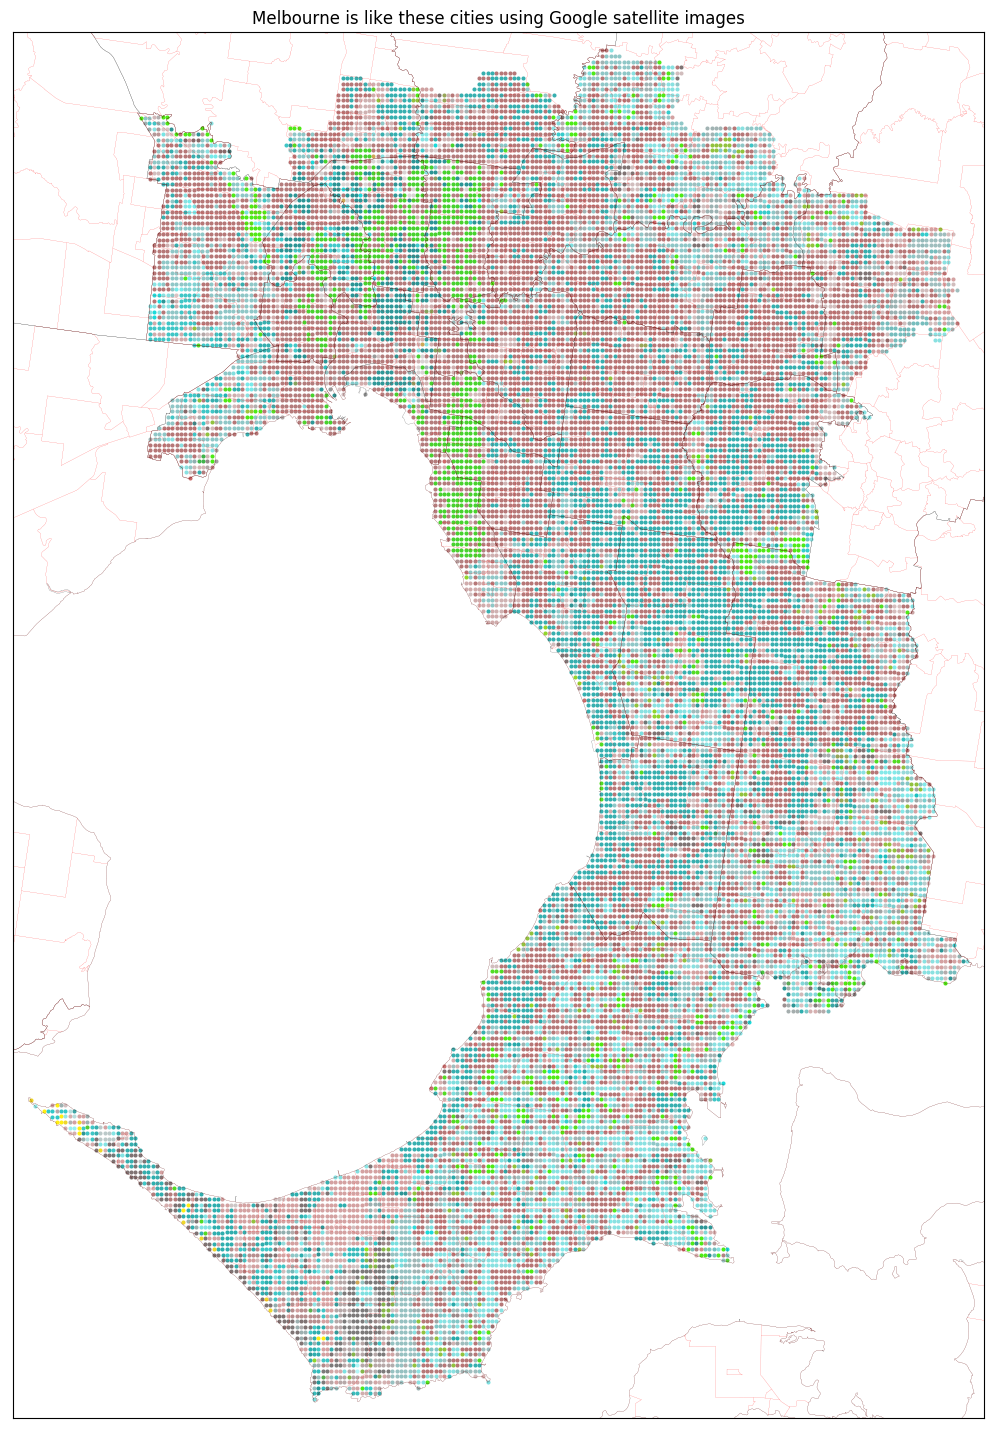
\includegraphics[scale=0.20]{Images/MelbourneOverall_sat.png} 
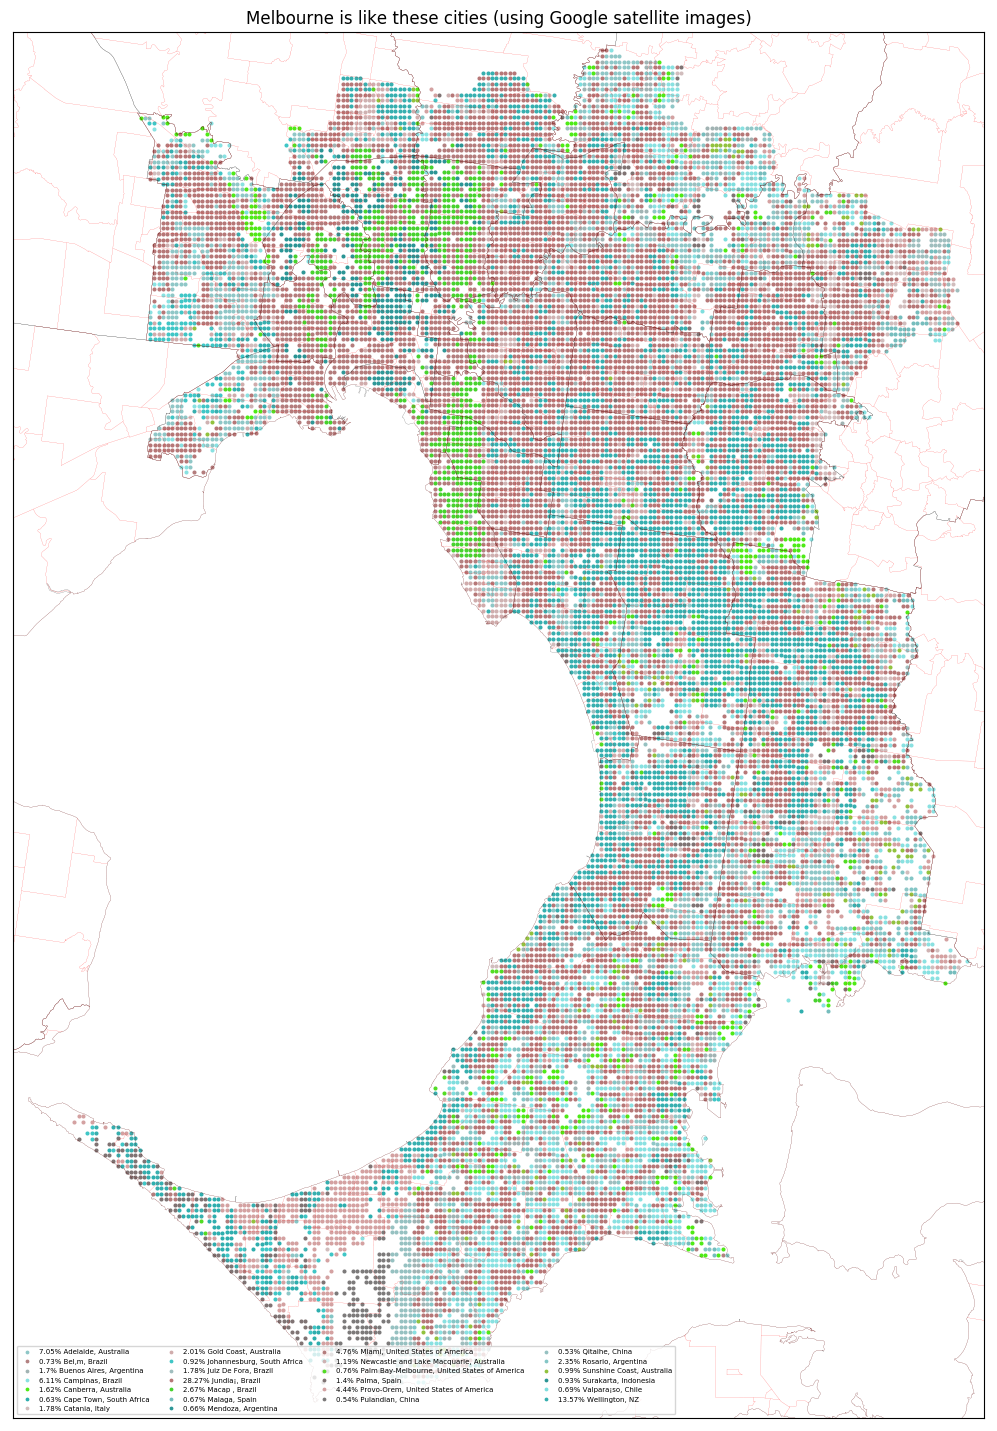
\includegraphics[scale=0.20]{Images/MelbourneOverallAbrev_sat.png} 
\caption{Predicted similar cities using GS neural network for Melbourne evaluation locations. All 1688 cities plotted using Figure \ref{fig:colorscheme} color scheme (left) and top 48 predicted cities (right)}    
 \label{fig:melsat}  
\end{figure} 



Figure \ref{fig:sydsat} shows all cities plotted against the Sydney evaluation locations as well as the top 48 predicted locations for the GS neural network. The overall predictions are dominated by cities in Brazil and other South American locations in the north and west and Ukraine in the south. Other Australian cities are only predicted in a few locations around the city. In the CBD, predictions continue to be dominated by Brazilian cities with some more scattered predictions of Japanese, Haiti, and Mexican cities. No predictions of Paris, France have been made by the GS neural network for any evaluation location in Sydney.



\begin{figure}[!htbp]
\centering    
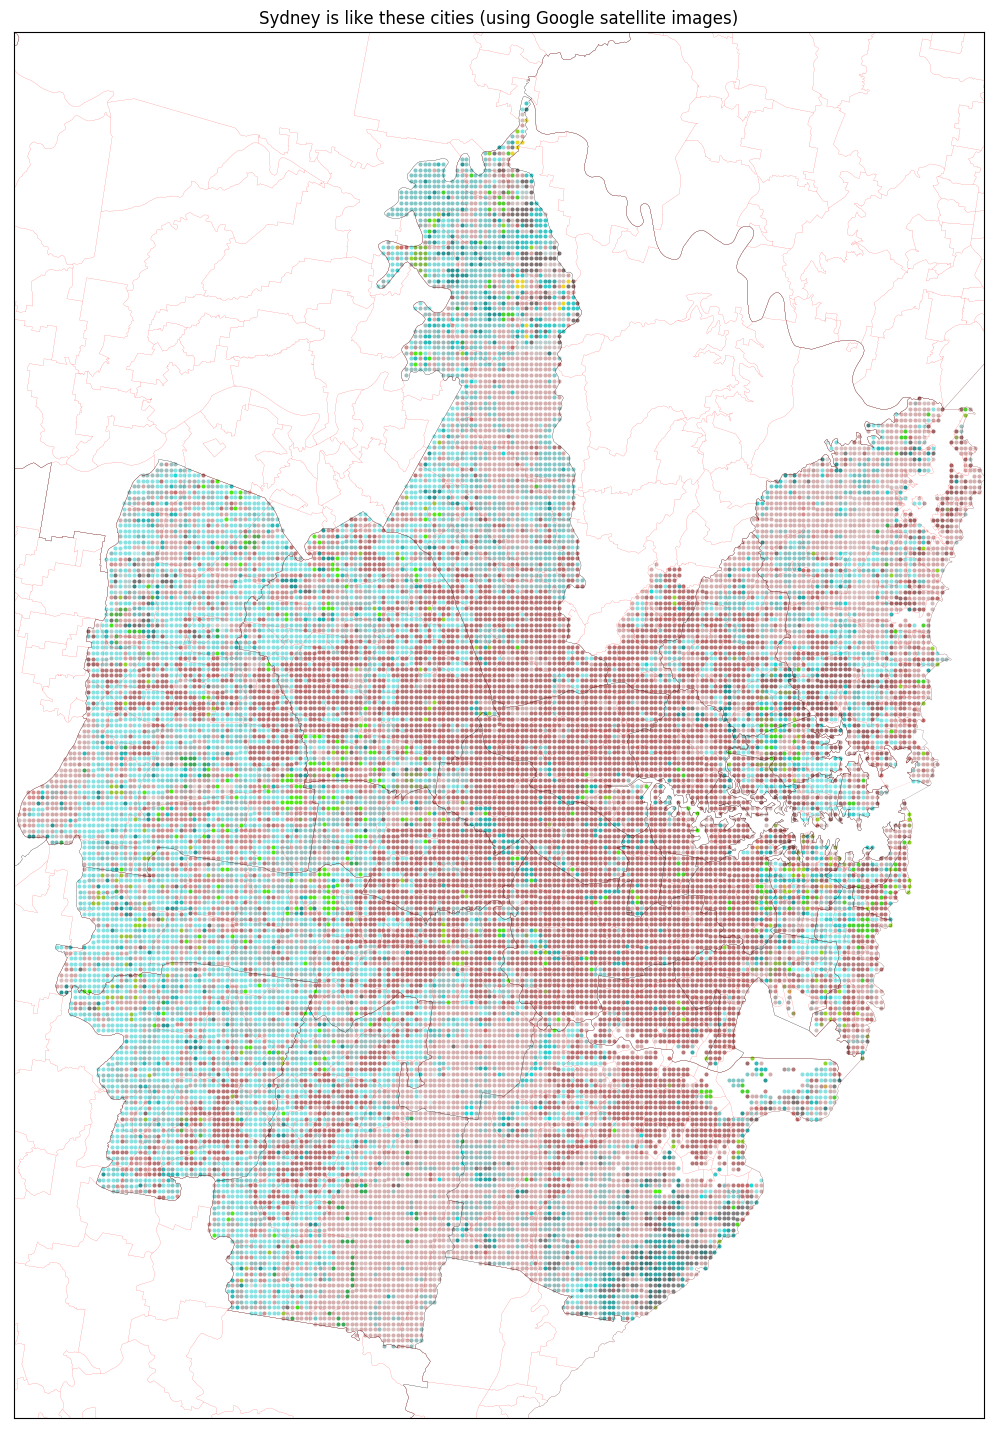
\includegraphics[scale=0.20]{Images/SydneyOverall_sat.png} 
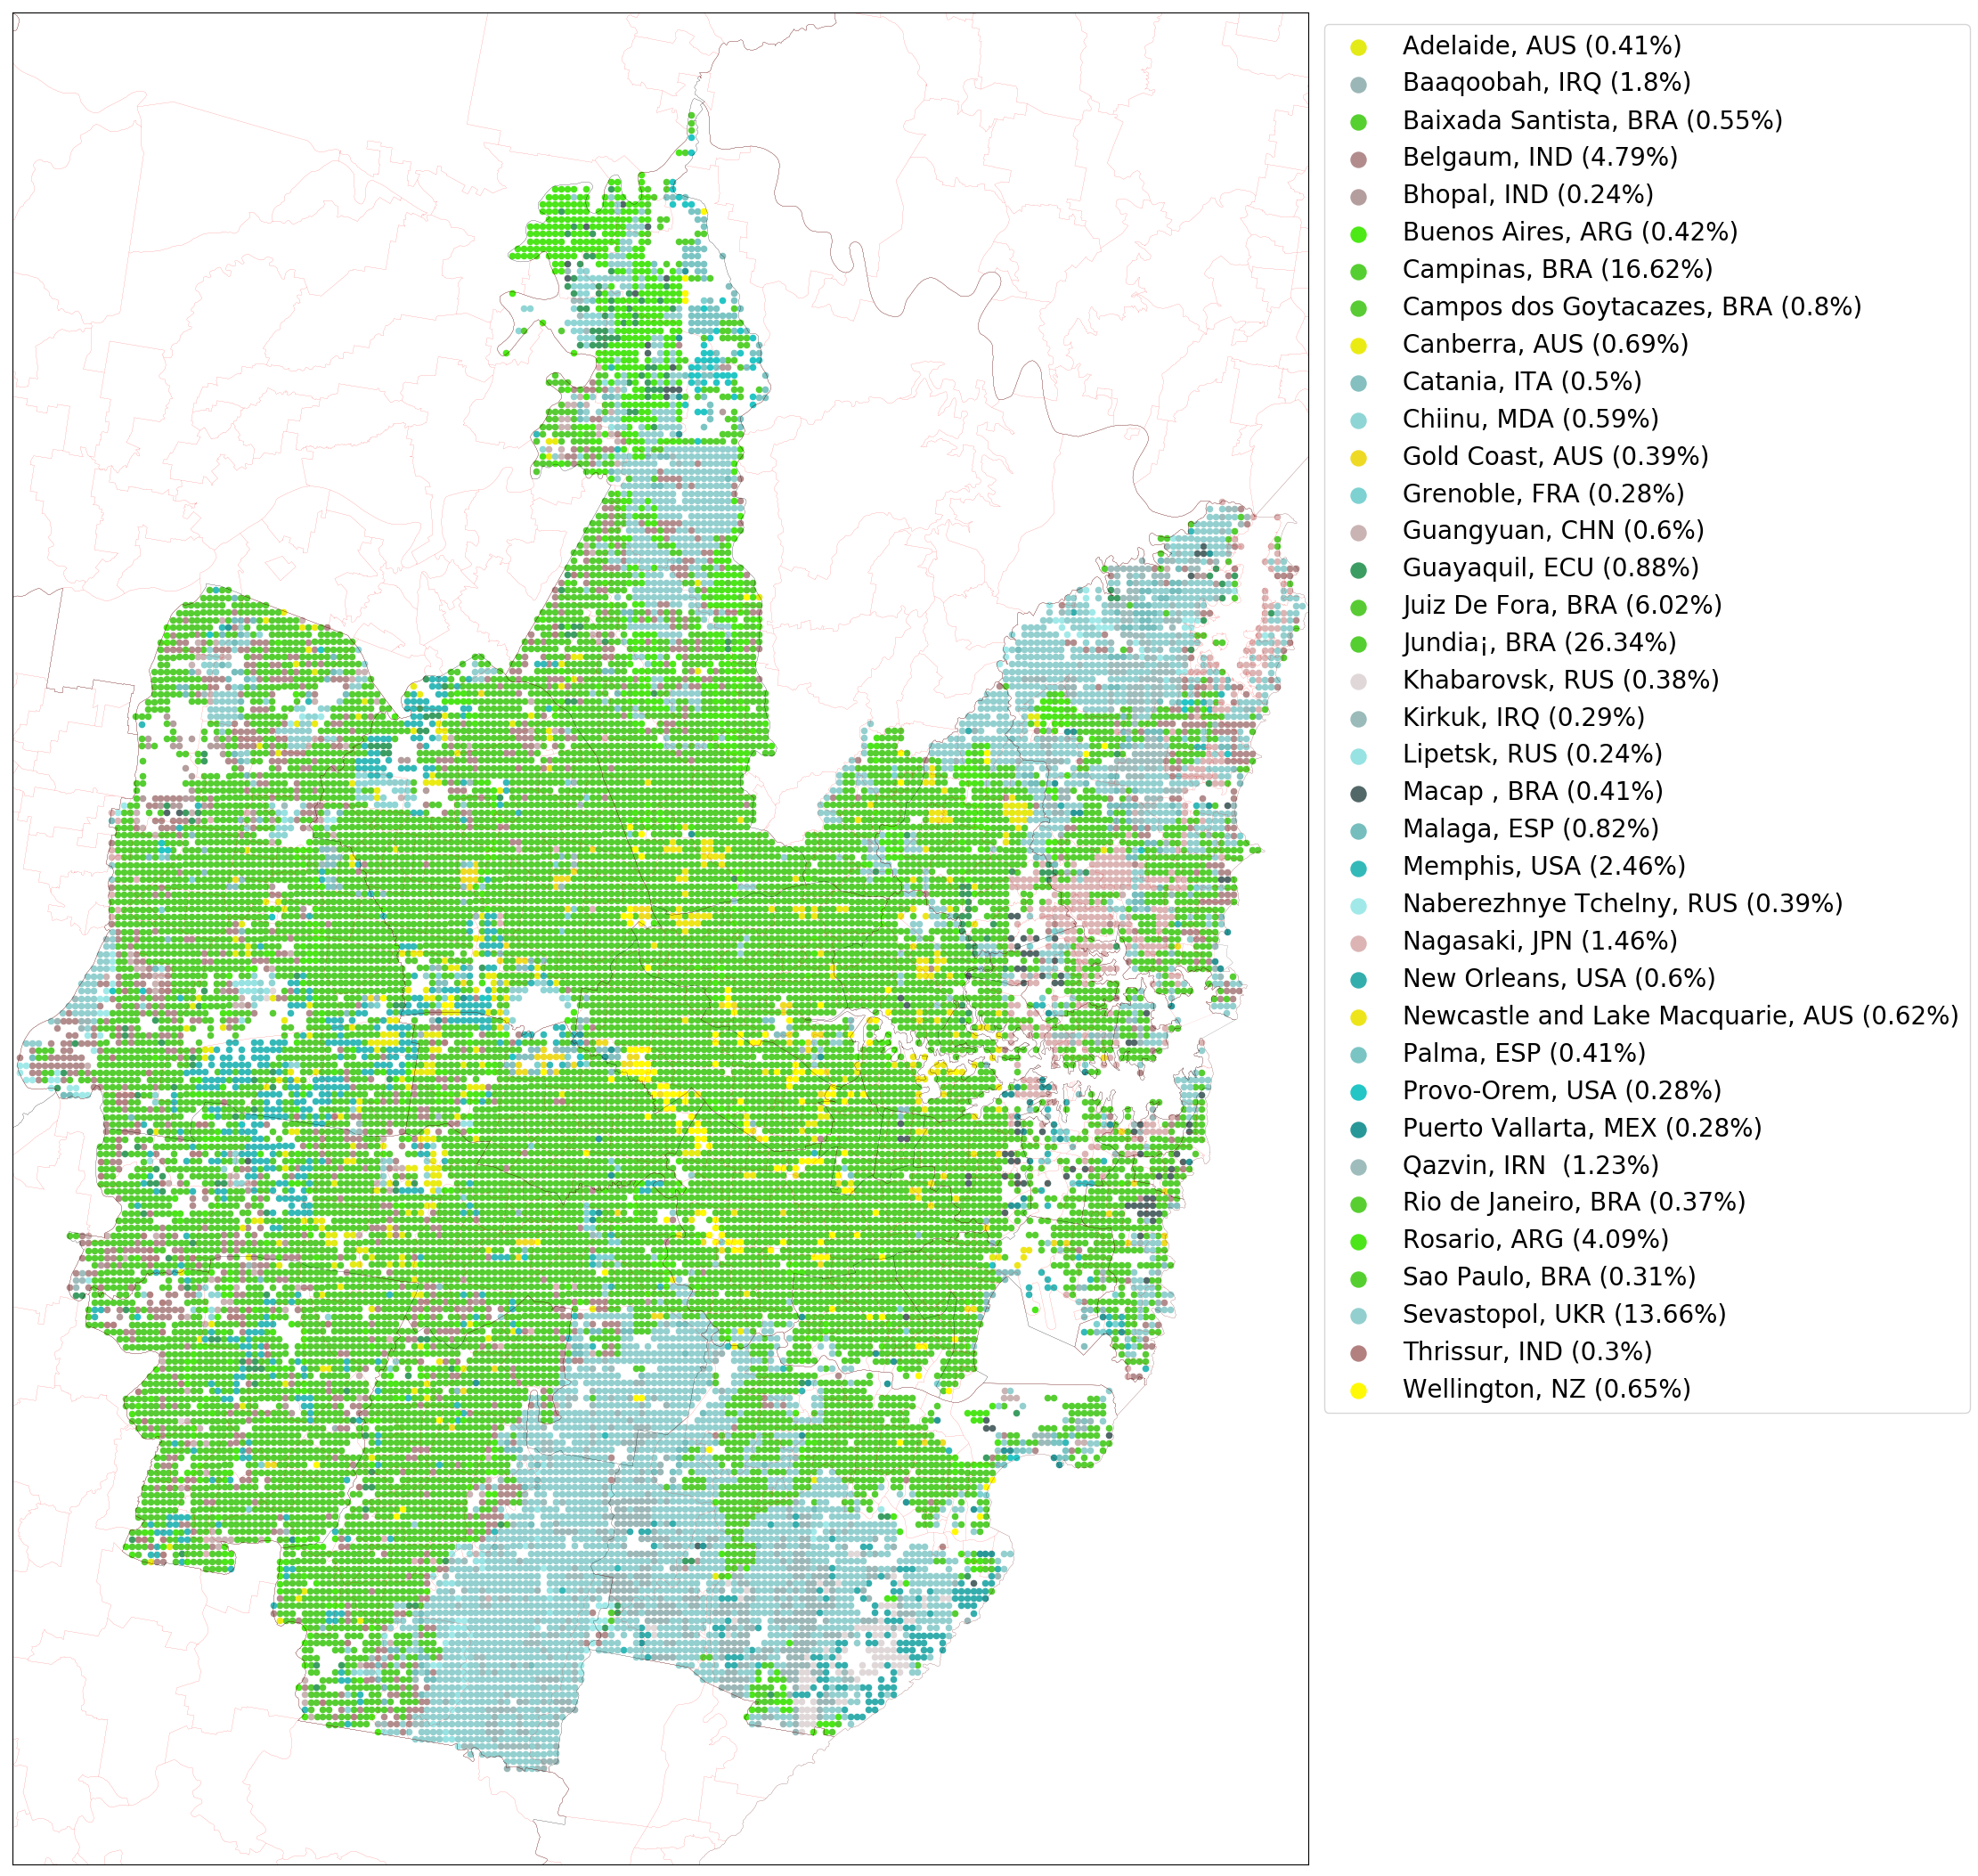
\includegraphics[scale=0.20]{Images/SydneyOverallAbrev_sat.png} 
\caption{Predicted similar cities using GS neural network for Sydney evaluation locations. All 1688 cities plotted using Figure \ref{fig:colorscheme} color scheme (left) and top 48 predicted cities (right)}    
 \label{fig:sydsat}  
\end{figure} 



Figure \ref{fig:melstreet} shows all cities plotted against the Melbourne evaluation locations as well as the top 29 predicted locations for the GSV-BSV neural network. The overall predictions are dominated by other Australian cities scattered widely throughout the entire greater Melbourne area. The remaining predicted results show no strong groupings of any predicted countries or cities but some of the common predictions include cities from South Africa, New Zealand, the United States, and European countries. The CBD again shows a wide scattering of predictions with no single city or country dominating. Only 13 predictions (out of 20971 evaluated locations) where made of Paris, France by the GSV-BSV neural network (Figure \ref{fig:gsv_melsyd_paris}).

\begin{figure}[!htbp]
\centering    
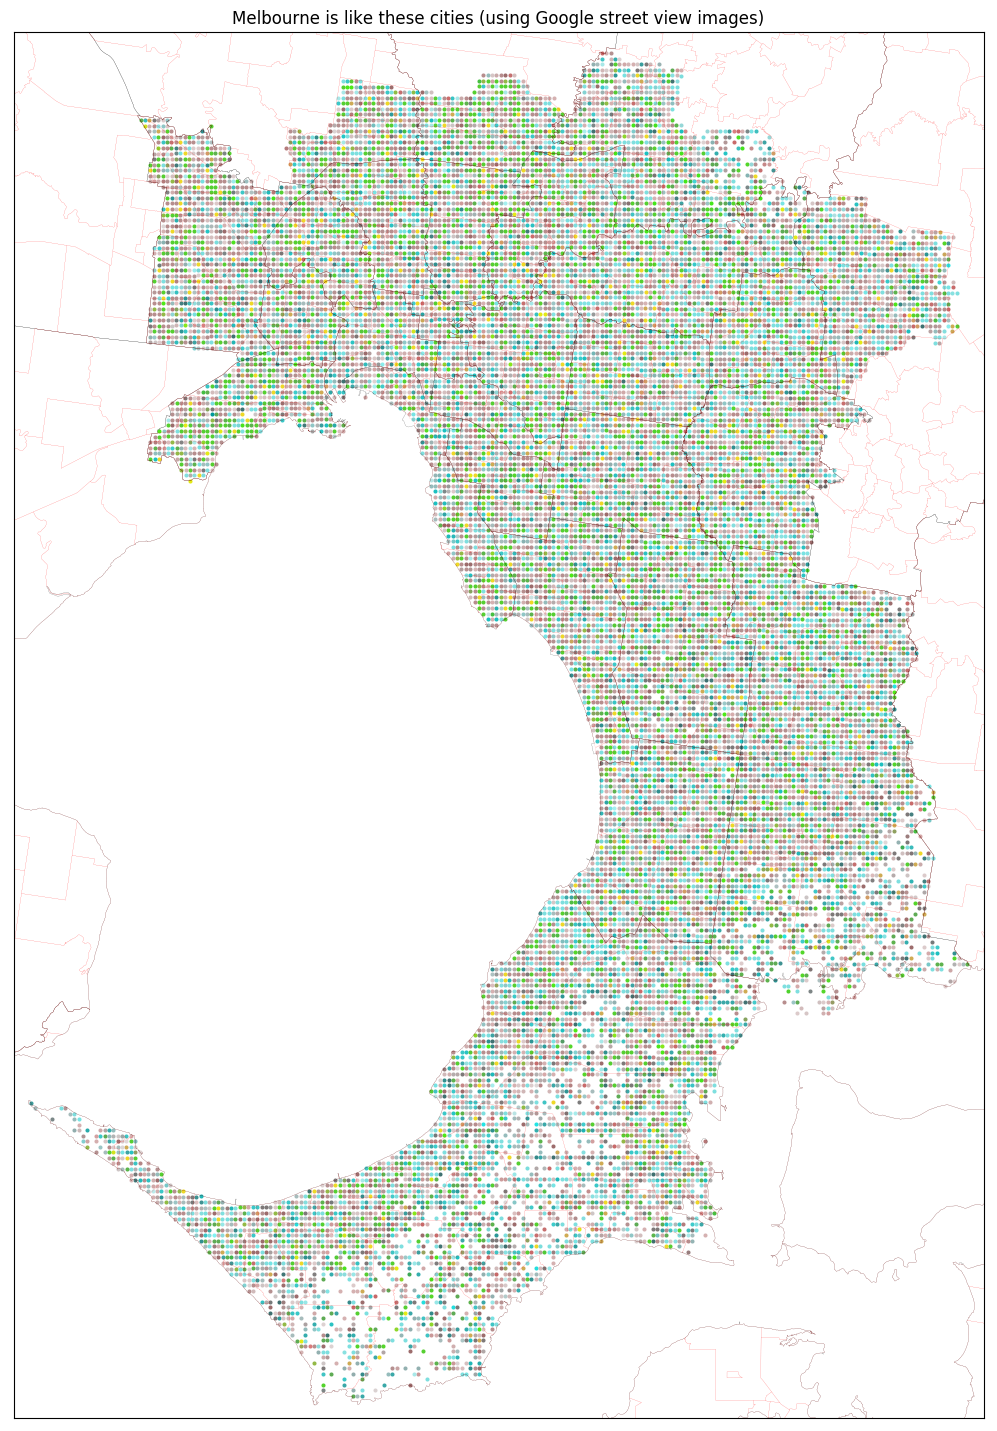
\includegraphics[scale=0.20]{Images/MelbourneOverall_street.png} 
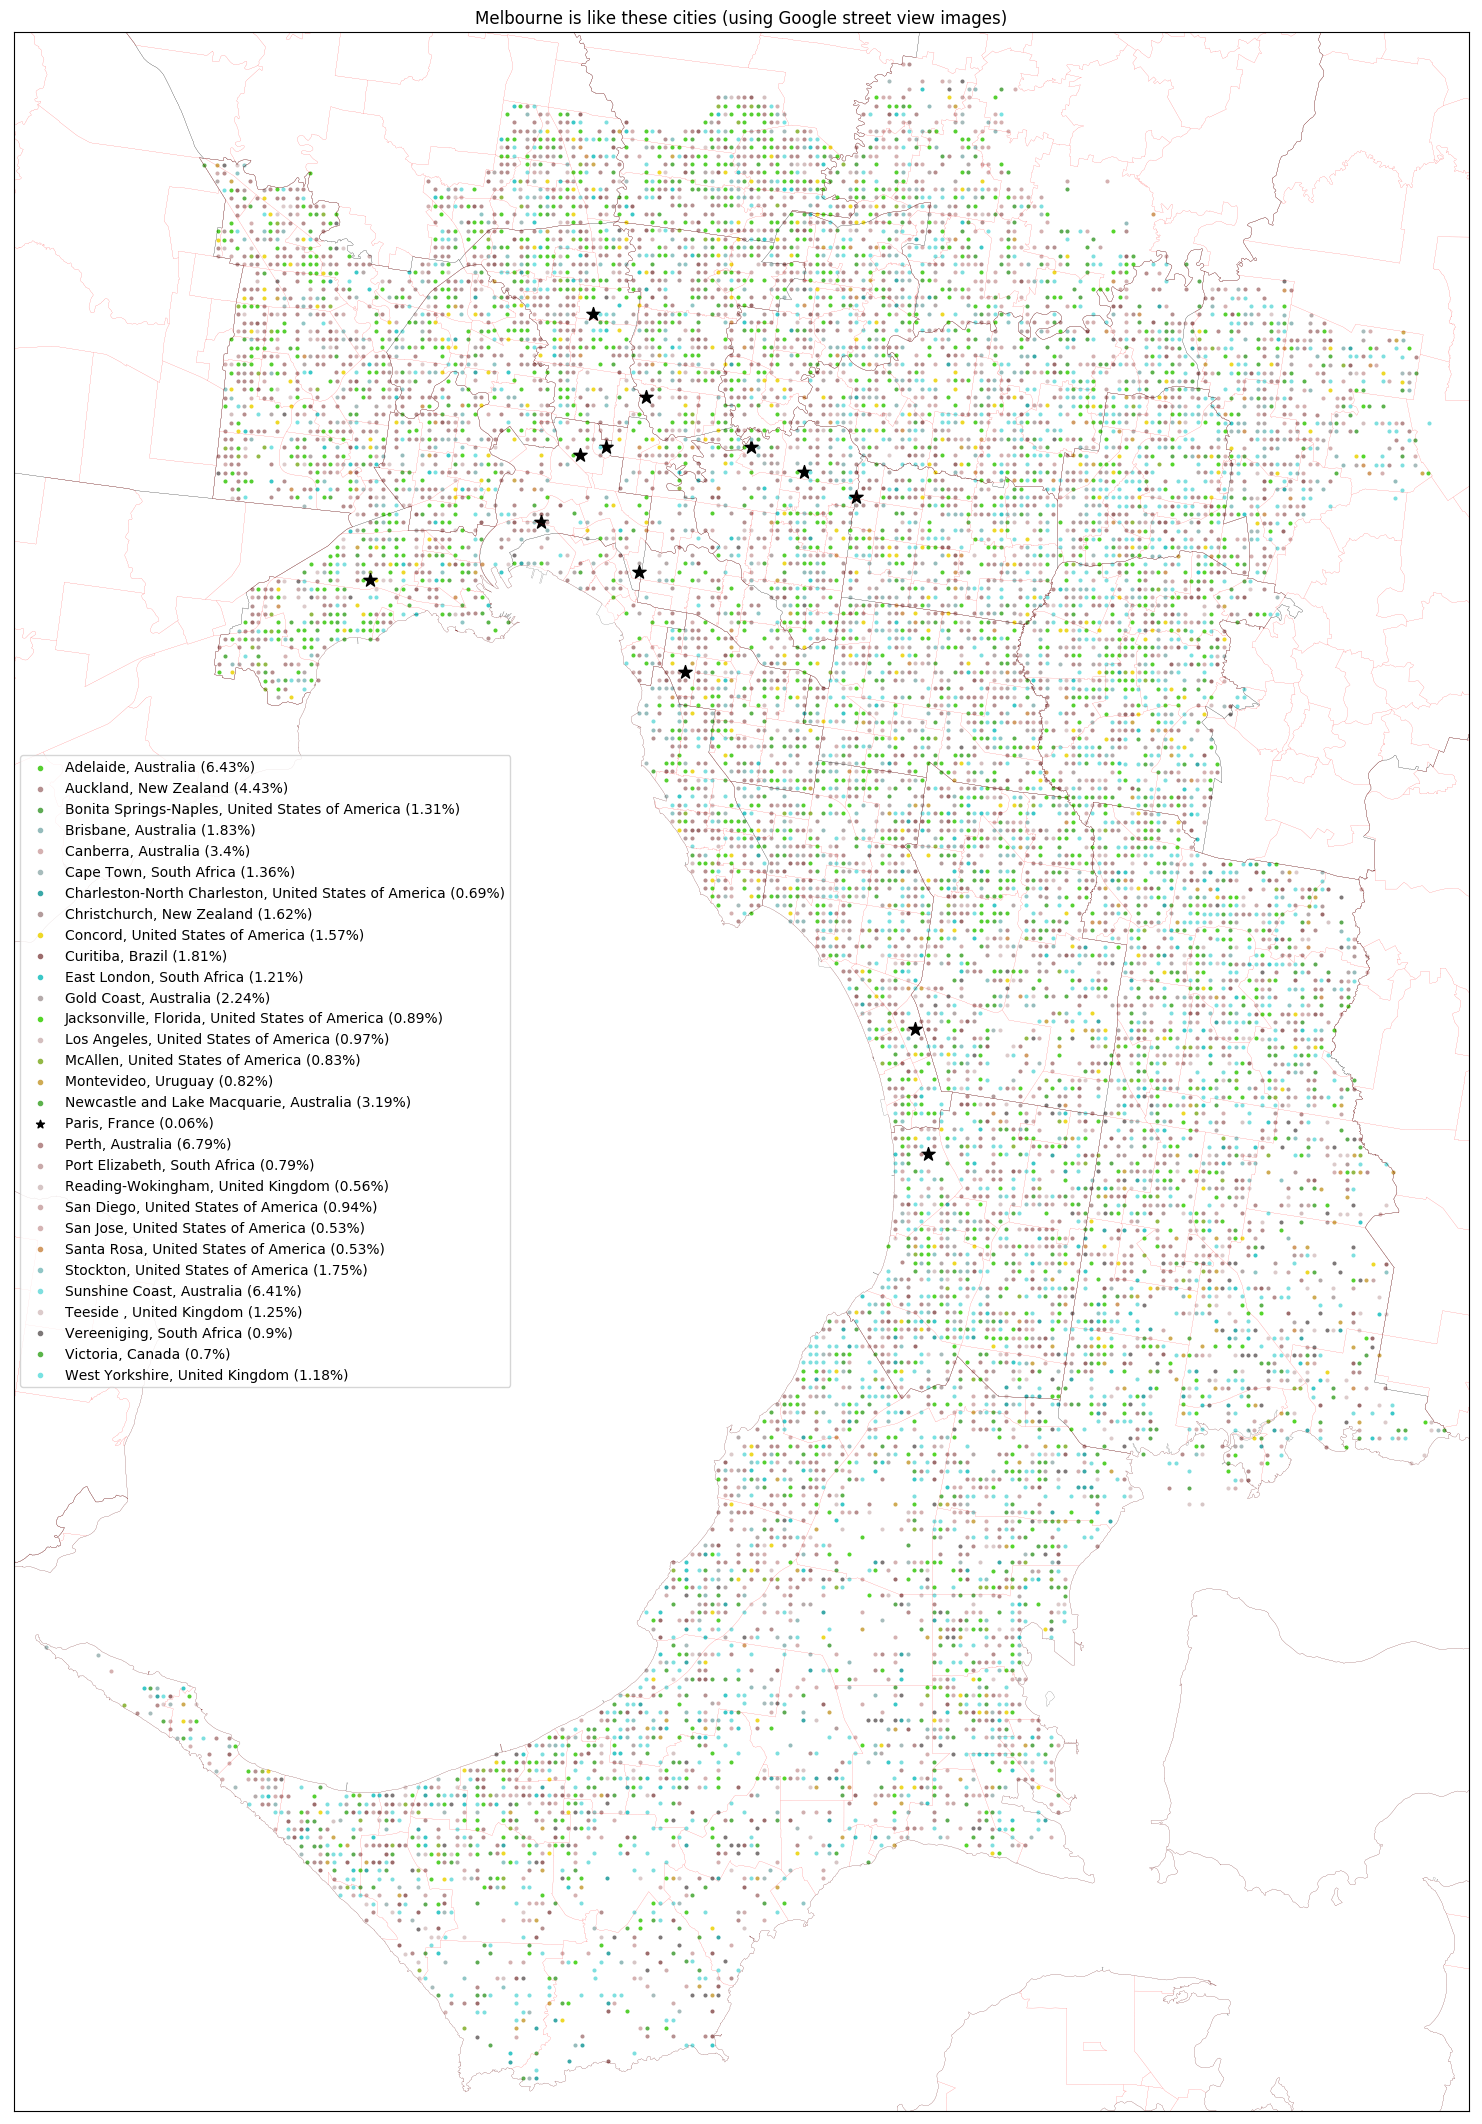
\includegraphics[scale=0.20]{Images/MelbourneOverallAbrev_street.png} 
\caption{Predicted similar cities using GSV-BSV neural network for Melbourne evaluation locations. All 1074 cities plotted using Figure \ref{fig:colorscheme} color scheme (left) and top 29 predicted cities (right)}    
 \label{fig:melstreet}  
\end{figure} 

\begin{figure}[!htbp]
\centering    
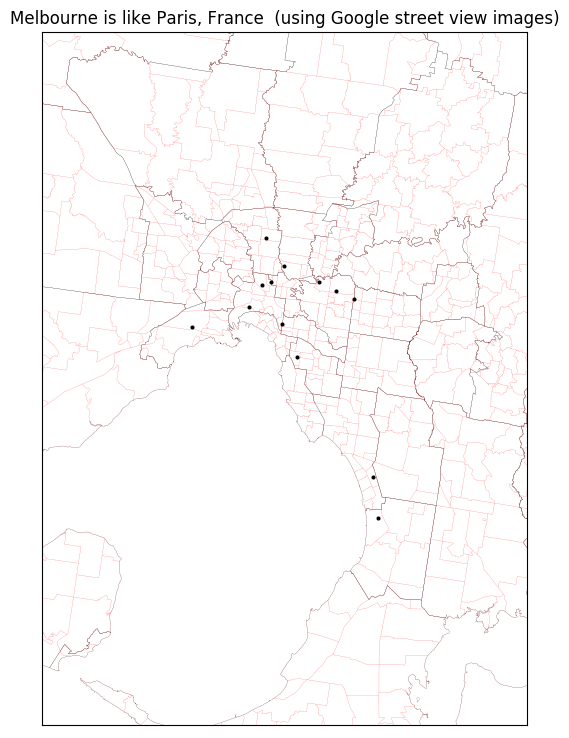
\includegraphics[scale=0.40]{Images/Melbourne_Paris,France-GSV.png} 
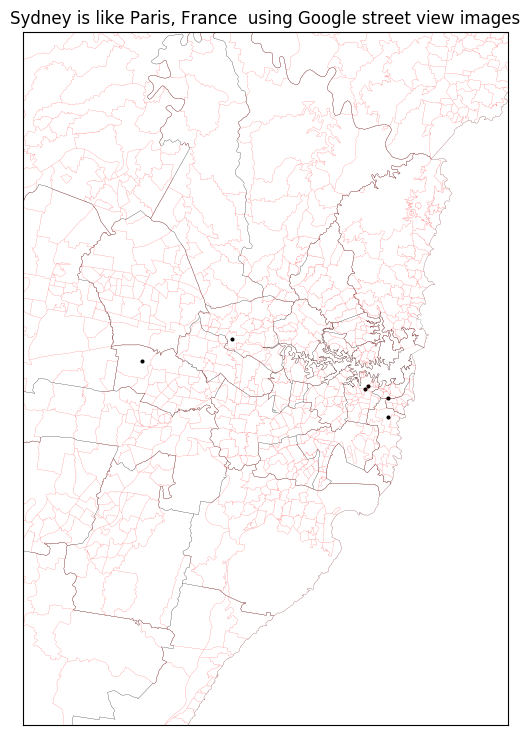
\includegraphics[scale=0.40]{Images/Sydney_Paris,France-GSV.png} 
\caption{Distribution of Paris predictions in Melbourne and Sydney using GSV-BSV.}    
 \label{fig:gsv_melsyd_paris}  
\end{figure}


Figure \ref{fig:sydstreet} shows all cities plotted against the Sydney evaluation locations as well as the top 29 predicted locations for the GSV-BSV neural network. The results are very similar to those in the Melbourne evaluation. Again, the overall predictions are dominated by other Australian cities scattered widely throughout the entire greater Sydney area. The remaining predicted results show no strong groupings of any predicted countries or cities but some of the common predictions include cities from the United States, New Zealand, South African, and a number of European countries. The CBD shows a similar scattering of predictions with no single city or country dominating (apart from other Australian cities). Only 6 predictions (out of 14644 evaluated locations) were made of Paris, France by the GSV-BSV neural network (Figure \ref{fig:gsv_melsyd_paris}).

\begin{figure}[!htbp]
\centering    
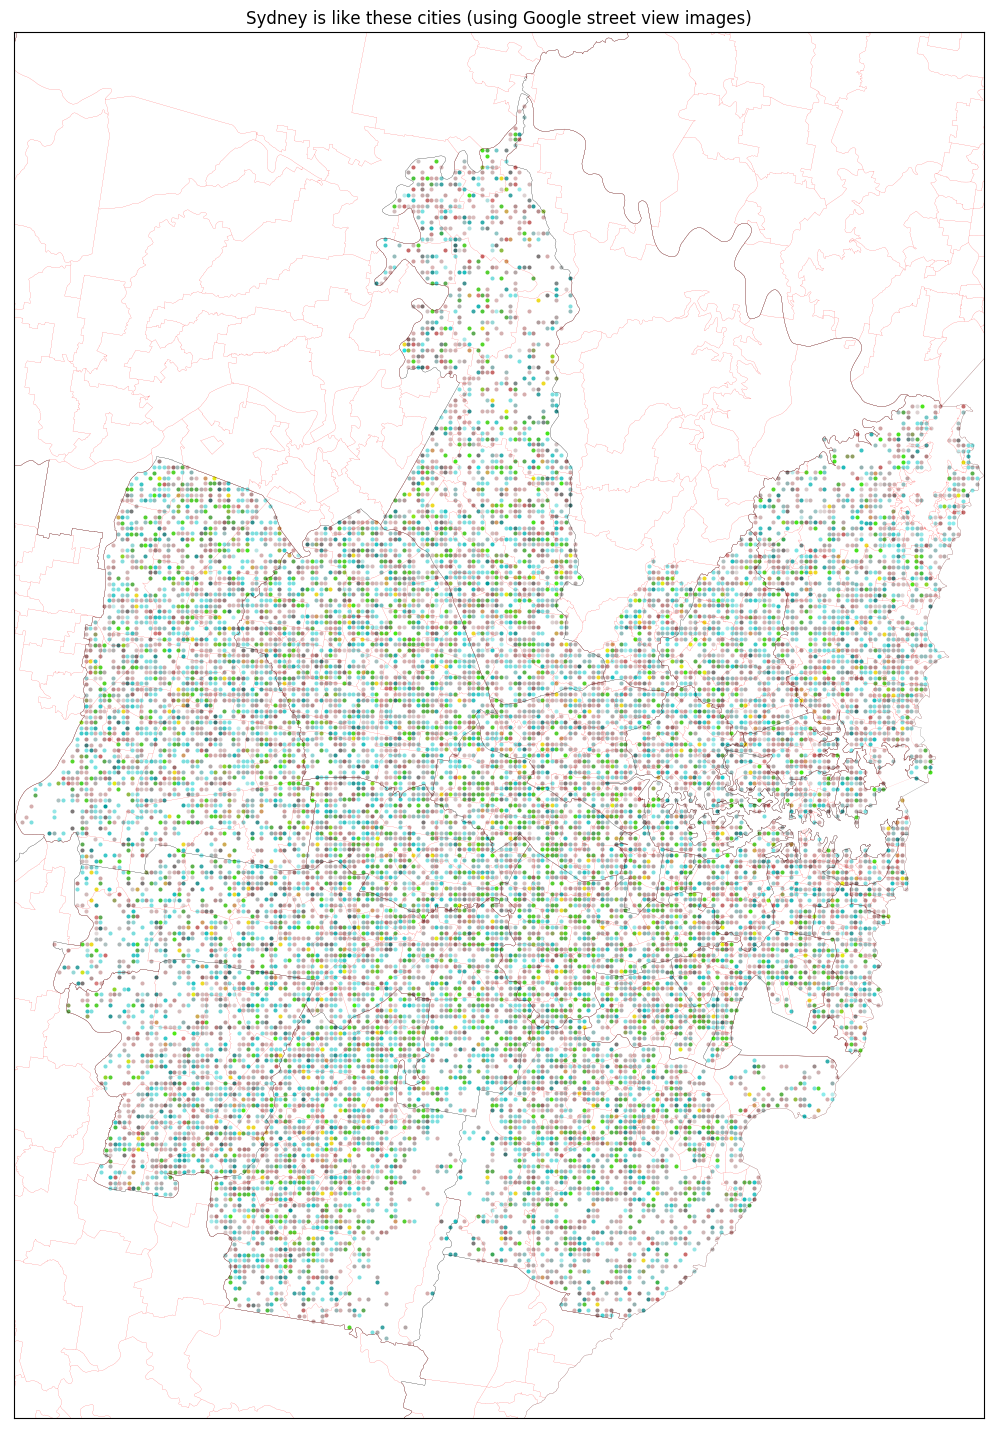
\includegraphics[scale=0.20]{Images/SydneyOverall_street.png} 
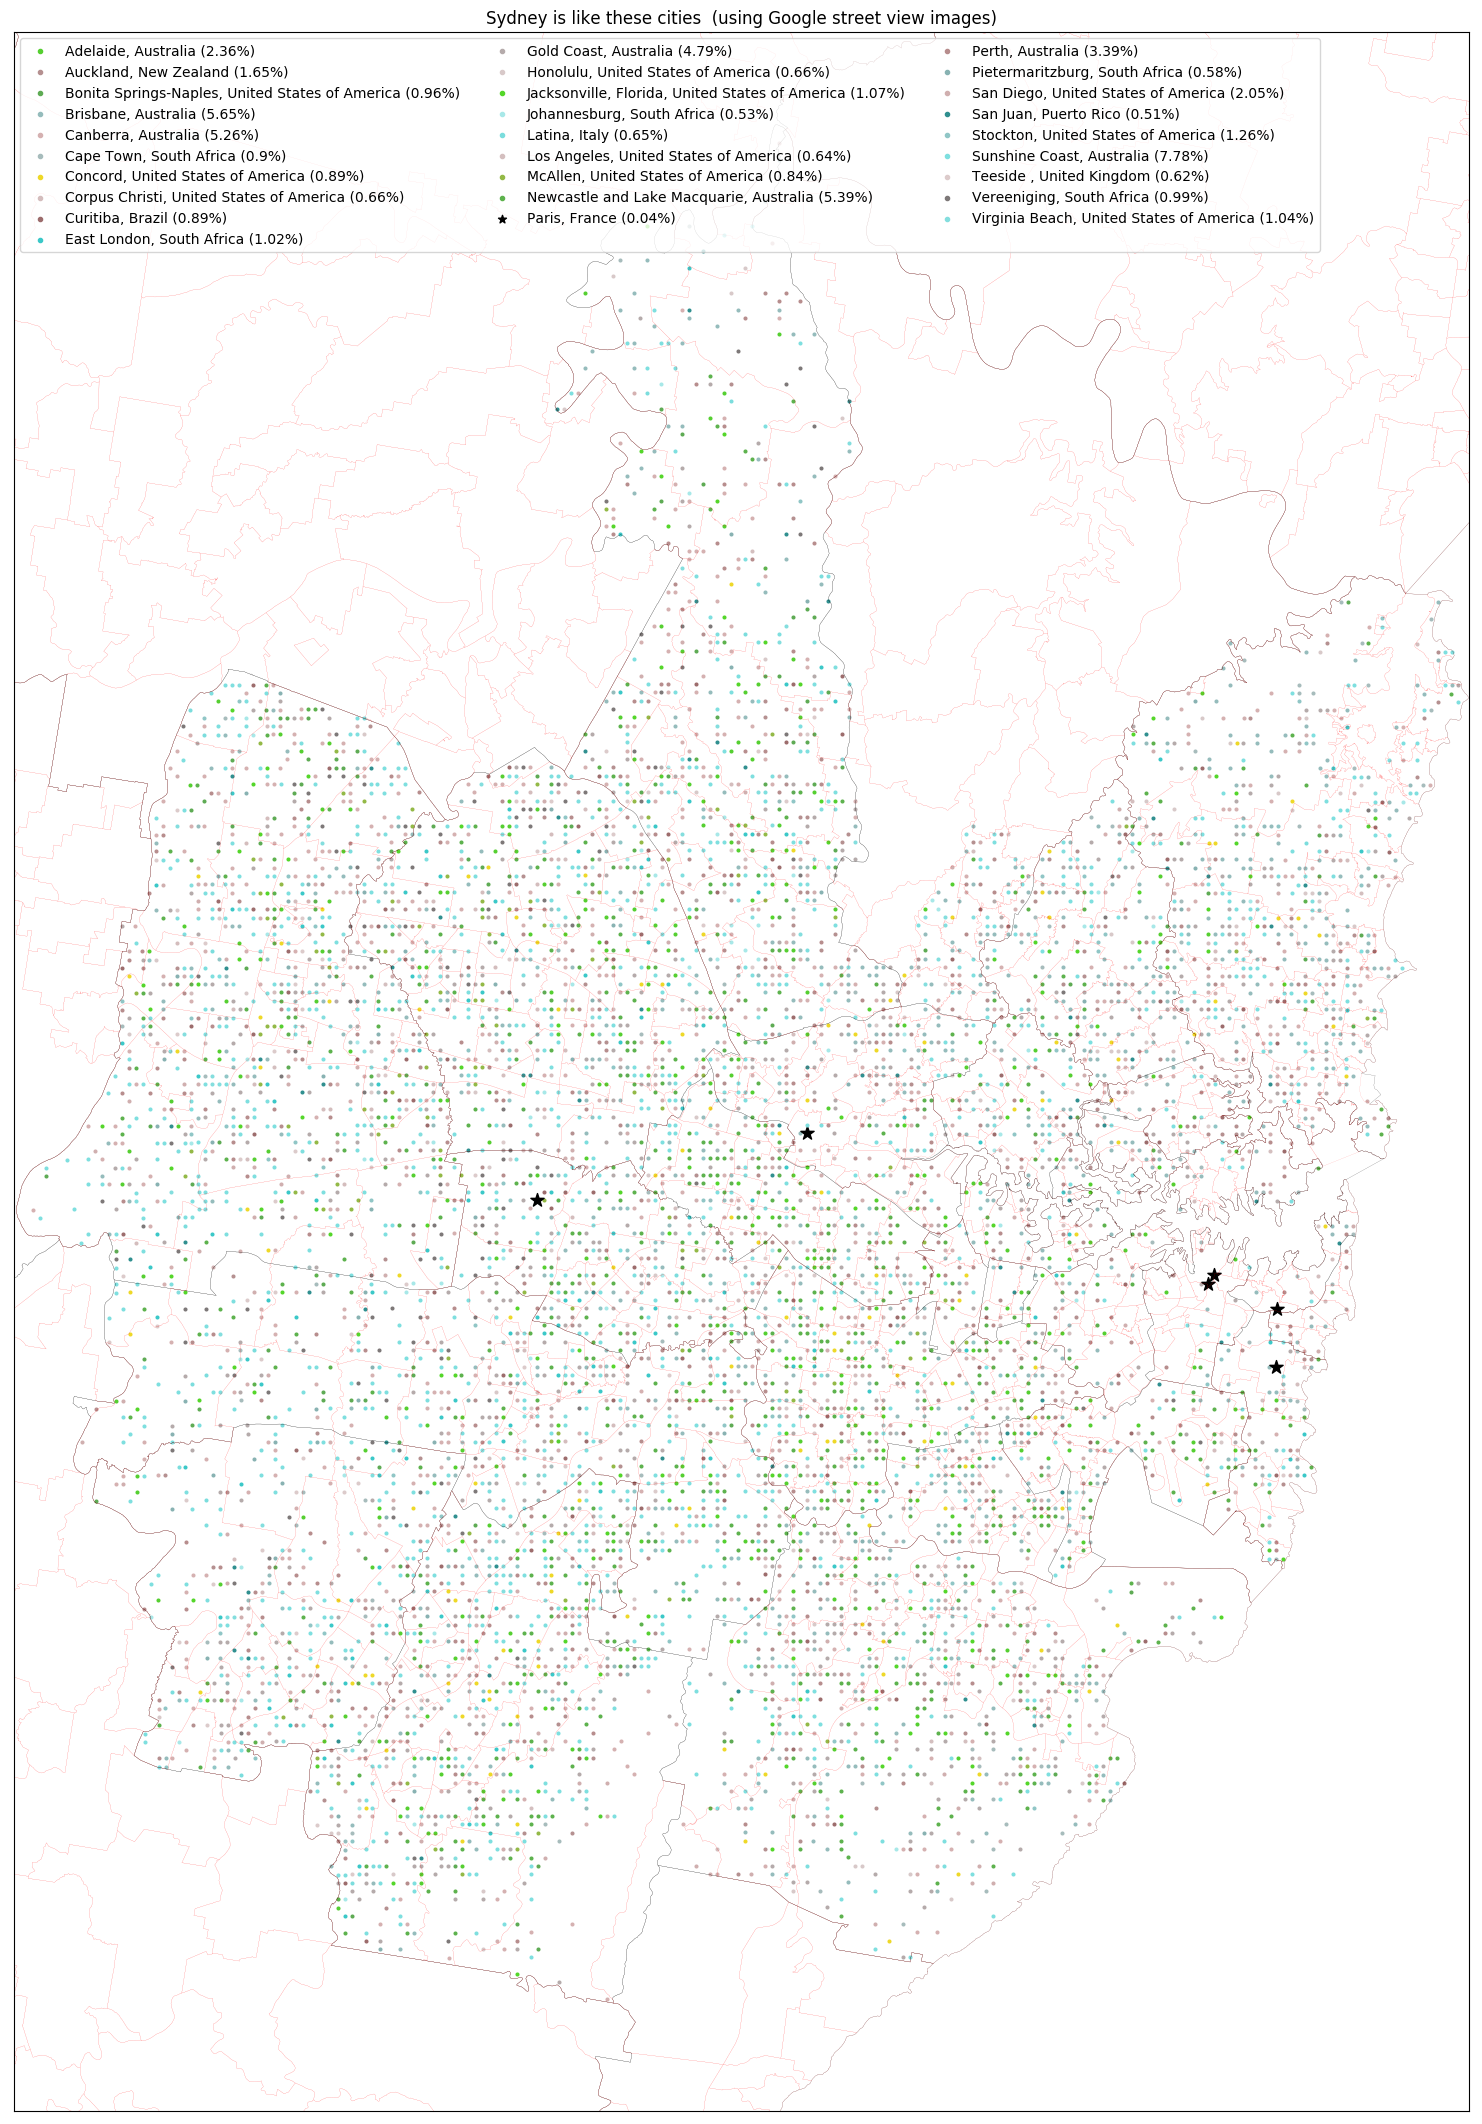
\includegraphics[scale=0.20]{Images/SydneyOverallAbrev_street.png}  
\caption{Predicted similar cities using GSV-BSV neural network for Sydney evaluation locations. All 1074 cities plotted using Figure \ref{fig:colorscheme} color scheme (left) and top 29 predicted cities (right)}    
 \label{fig:sydstreet}  
\end{figure} 


%\begin{figure}[!htbp]
%\centering    
%\includegraphics[scale=0.20]{Images/Melbourne_satellite_abr.png} 
%\includegraphics[scale=0.20]{Images/Sydney_satellite_abr.png} 
%\includegraphics[scale=0.20]{Images/Melbourne_maps_abr.png} 
%\includegraphics[scale=0.20]{Images/Sydney_maps_abr.png} 
%\includegraphics[scale=0.20]{Images/Melbourne_street_abr.png} 
%\includegraphics[scale=0.20]{Images/Sydney_street_abr.png} 
%\caption{Predicted similar country of predicted locations using GS, GM, and GSV-BSV neural networks for Melbourne and Sydney evaluation locations.}    
% \label{fig:gislabels}  
%\end{figure} 


\section{Discussion}\label{sec:discussion}
Paris, France is a widely recognizable international iconic city \citep{Anholt2006}, leading to many cities to claim that they have a `Paris-end' of town \citep{Williams2010}, or are a Paris on the \textless insert name of local river \textgreater \citep{Wilden2013}. Visual elements of Paris are widely recognizable \citep{Doersch2012} but can Melbourne or Sydney truly claim to have a `Paris-end' or is Melbourne `Paris on the Yarra' or Sydney `Paris on the Parramatta'? In this study, we use three neural networks, trained using three different visual data sources to test whether either Melbourne or Sydney can really make these claims. 

In addition to potentially making some local tourist boards unhappy, we also present a fundamental methodology to objectively analyse urban areas using big data imagery. We find that each of these data sources uncovers a unique set of urban typologies and that understanding the aims of each analysis requires and understanding of what parameters each data set will emphasise.

In the first issue, as the results section above show, we can conclusively disprove that either Melbourne and Sydney have a strong case to claim that they have large commonalities with Paris. Using the three different trained neural networks, Paris barely even registers as a prediction in evaluations of either Melbourne or Sydney locations. 

However, in looking at the predictions that do predict a Paris match, there are a number of characteristics about Paris that stand out. A gallery of all of the images for Melbourne and Sydney that the GM neural network found were similar to Paris (Figures \ref{fig:gm_mel_gallery} and \ref{fig:gm_syd_gallery}) shows many common elements. Many of these map images show large parklands (in green) embedded in the cities. Orange lines of public transport (rail and tram) are prominent in the majority of these images as well as large water bodies (in blue). Large arterial and trunk roads run nearby smaller (often curving) local roads, however these local roads tend to still be larger and do not reach the small intricate layouts of some Asian cities.

 \begin{figure}[!htbp]
 \centering    
 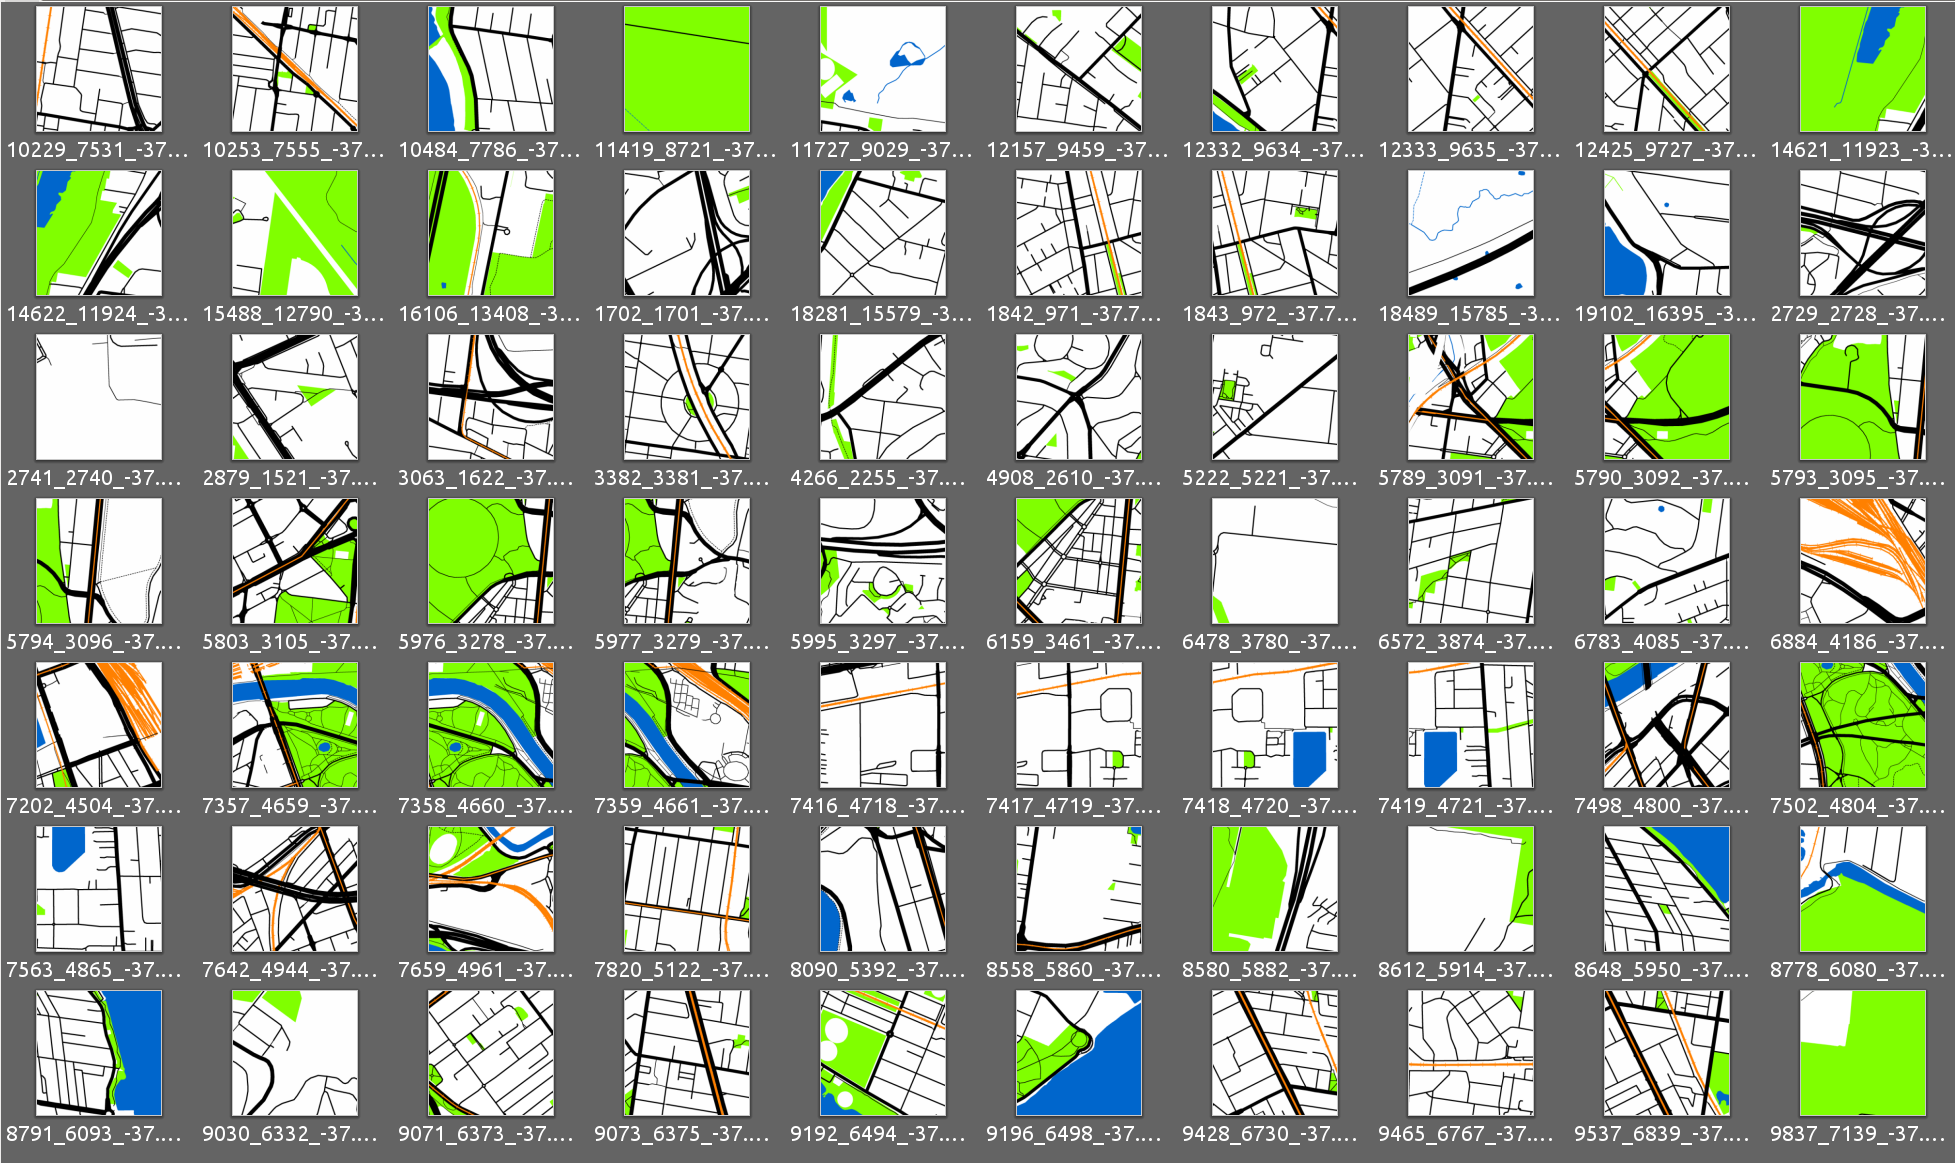
\includegraphics[scale=0.50]{Images/MelbourneLikeParis/Melbourne_maps_gallery.png} 
 \caption{Gallery of Paris predictions for Melbourne using GM.}    
  \label{fig:gm_mel_gallery}  
 \end{figure} 

\begin{figure}[!htbp]
\centering    
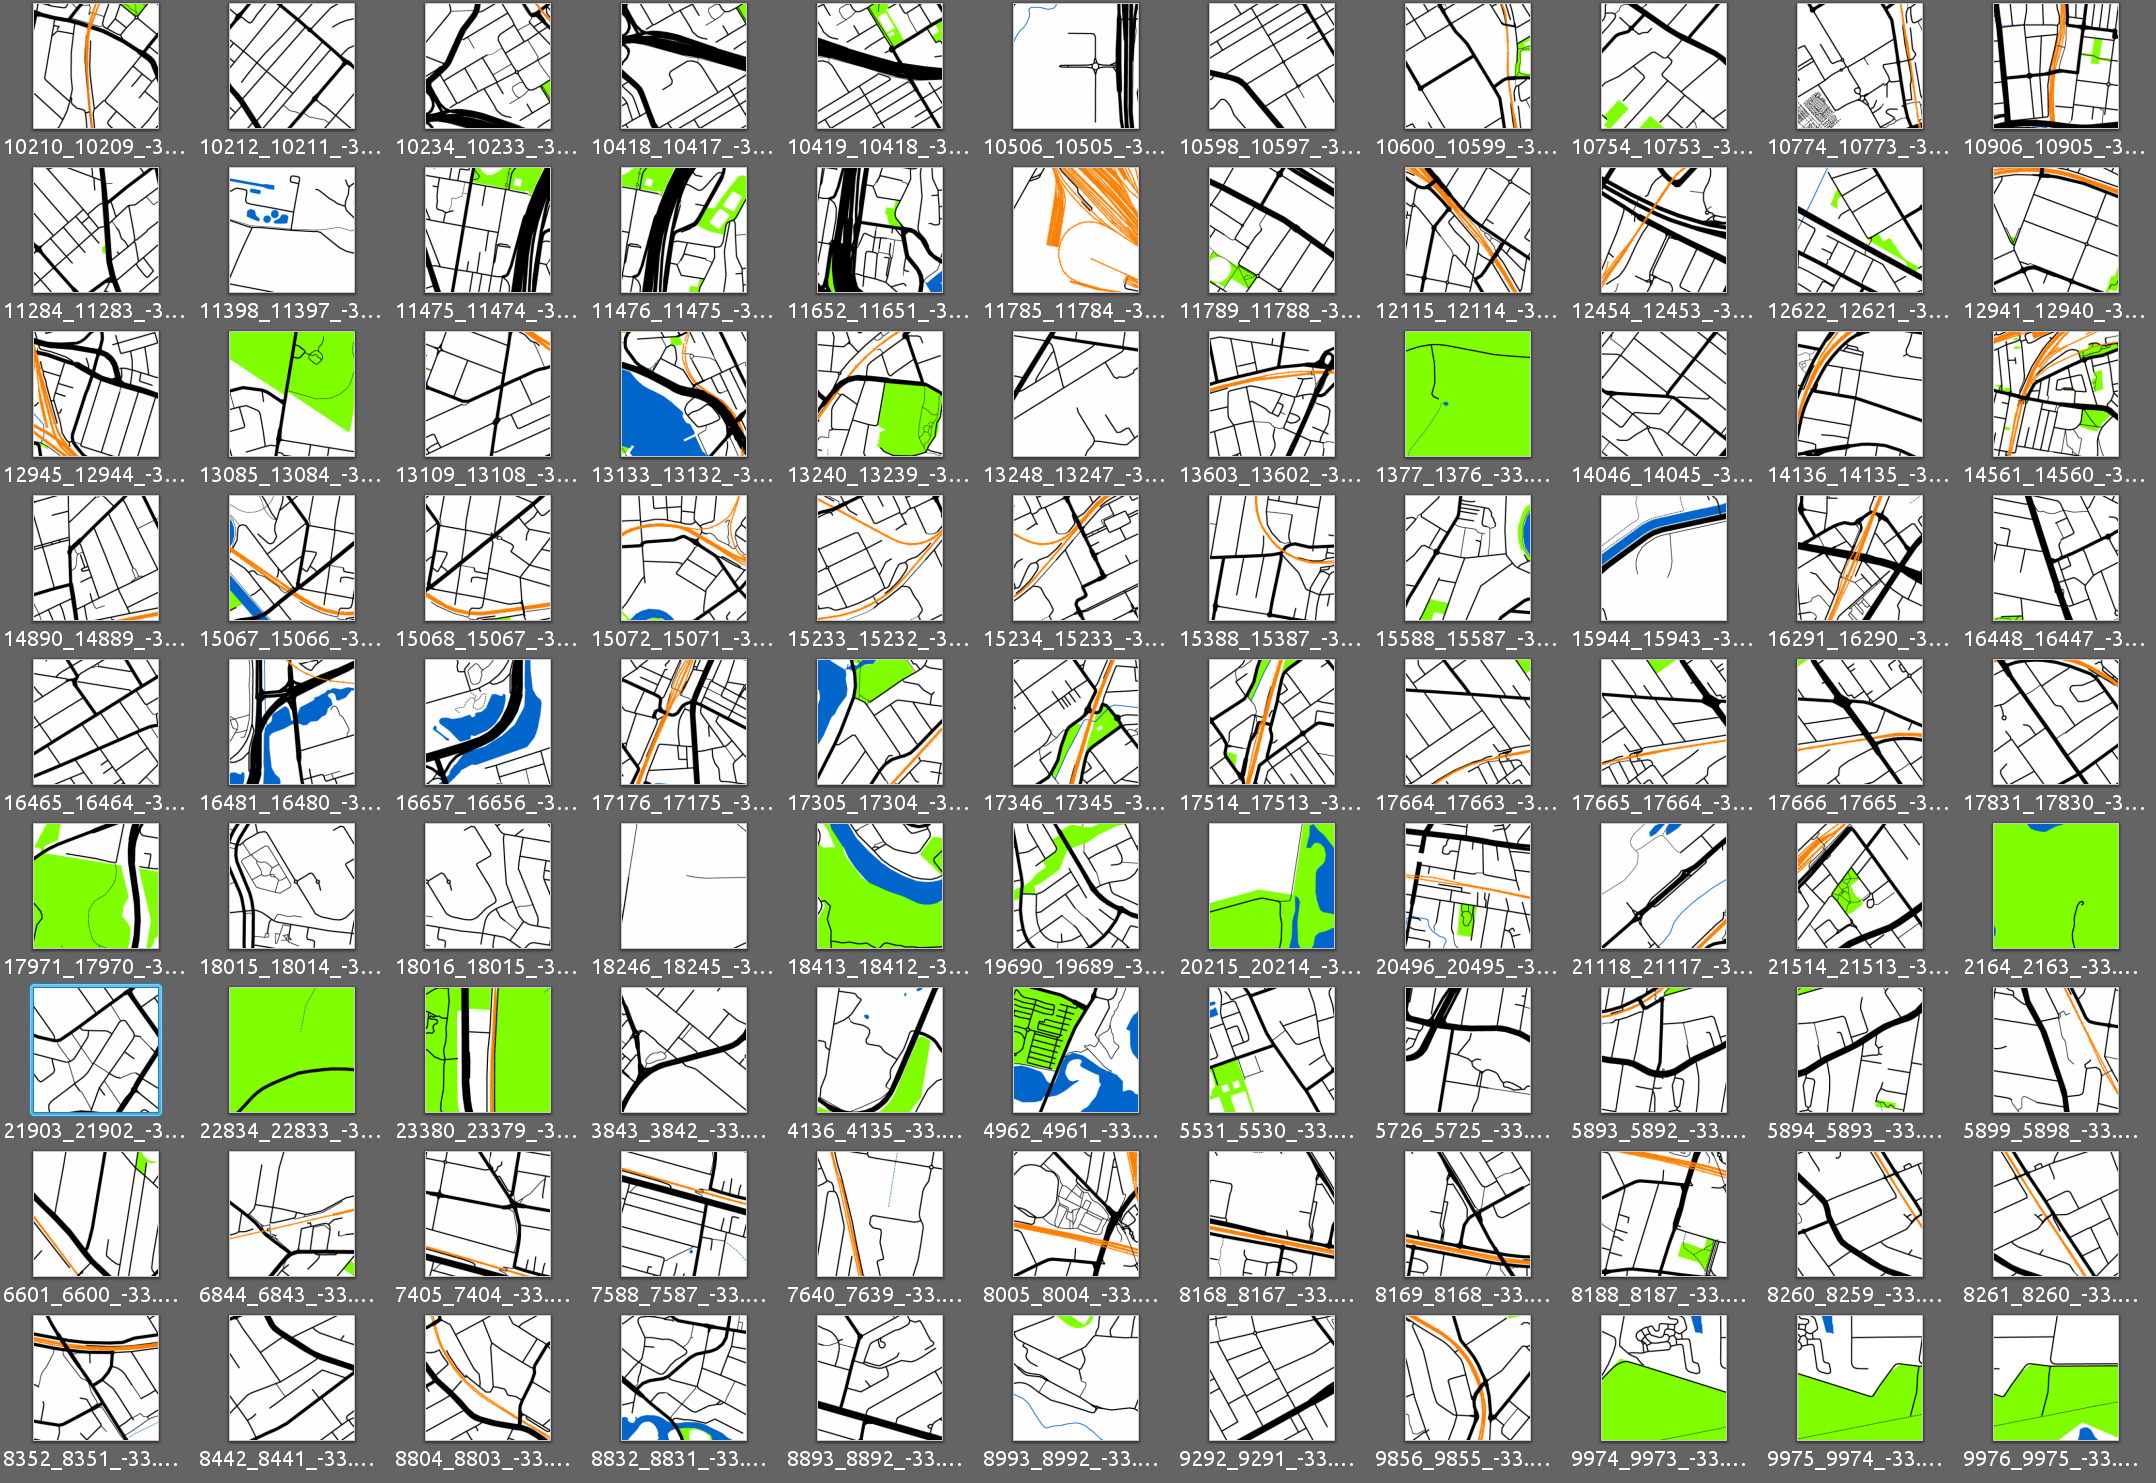
\includegraphics[scale=0.50]{Images/SydneyLikeParis/Sydney_maps_gallery.png} 
\caption{Gallery of Paris predictions for Sydney using GM.}    
 \label{fig:gm_syd_gallery}  
\end{figure} 

As the GSV-BSV neural network only picked Paris for 0.062\% of the evaluated locations for Melbourne and 0.40\% for Sydney, it can be stated that from a visual street-level view, there is almost nothing about either Melbourne or Sydney that is visually similar to Paris. In the very few predicted locations that were predicted to be Paris (Figures \ref{fig:gsv_mel_gallery} and  \ref{fig:gsv_syd_gallery}), it can only be inferred that perhaps street trees are an important part of what makes Paris look like Paris.





\begin{figure}[!htbp]
\centering    
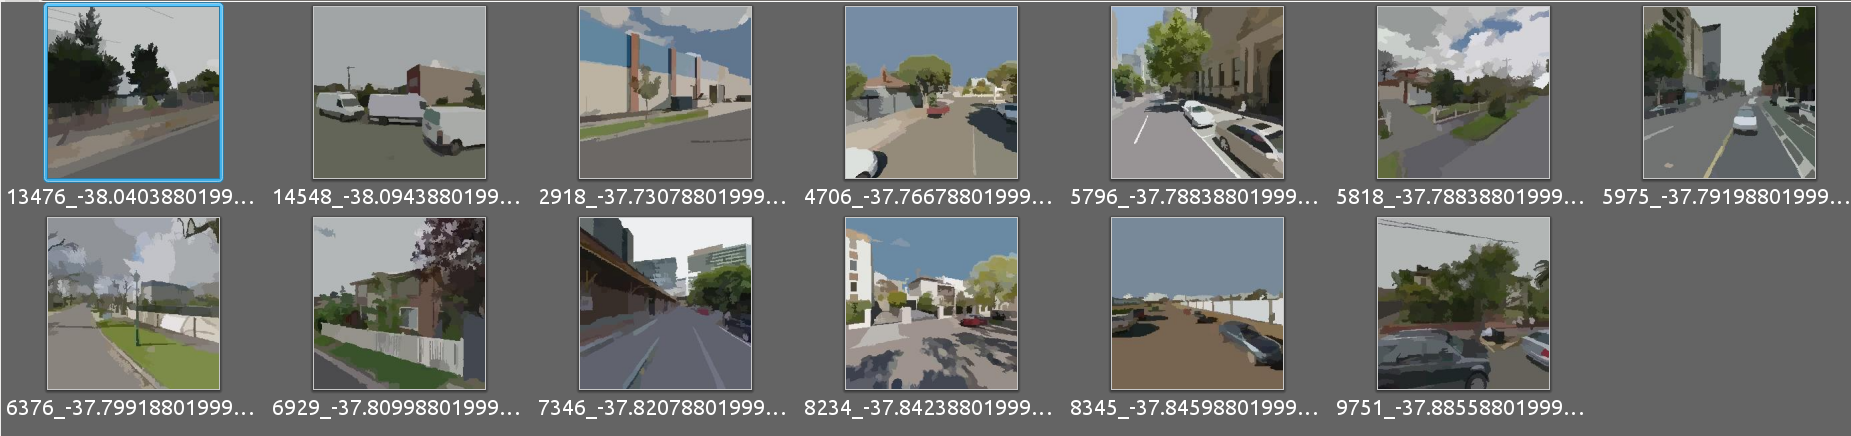
\includegraphics[scale=0.50]{Images/MelbourneLikeParis/Melbourne_streetview_gallery.png} 
\caption{Gallery of Paris predictions for Melbourne using GSV-BSV.}    
 \label{fig:gsv_mel_gallery}  
\end{figure} 

\begin{figure}[!htbp]
\centering    
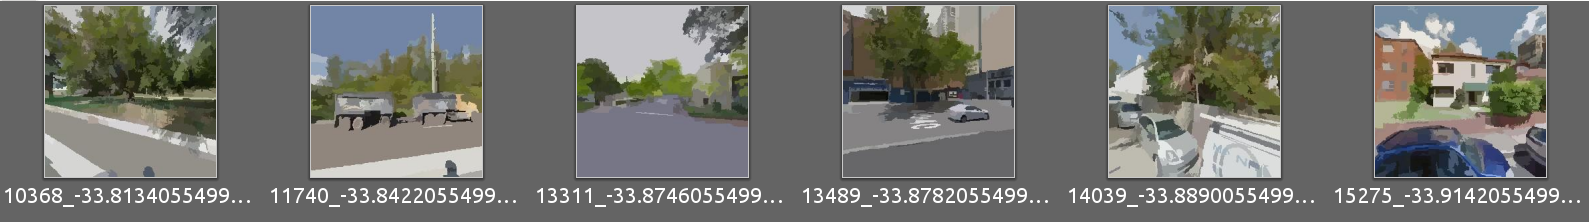
\includegraphics[scale=0.50]{Images/SydneyLikeParis/Sydney_streetview_gallery.png} 
\caption{Gallery of Paris predictions for Sydney using GSV-BSV.}    
 \label{fig:gsv_syd_gallery}  
\end{figure} 















A fundamental methodology to analyse urban areas. Understanding the goals of the typology and the data source, leading to 

Parameters lead to what sorts of results.










\section{Conclusion}\label{sec:conclusion}

%\begin{thebibliography}{}
%\subsection*{References}\label{sec:ref}

  %%Harvard (name/date)
  \bibliographystyle{SageH}
  %%Vancouver (numbered)
  %\bibliographystyle{SageV} 
  \bibliography{library}
%  \bibitem[ ()]{}
% \end{thebibliography} 


\end{document}

